\documentclass[a4paper]{book}
\usepackage{a4wide}
\usepackage{makeidx}
\usepackage{fancyhdr}
\usepackage{graphicx}
\usepackage{multicol}
\usepackage{float}
\usepackage{textcomp}
\usepackage{alltt}
\usepackage{times}
\usepackage{ifpdf}
\ifpdf
\usepackage[pdftex,
            pagebackref=true,
            colorlinks=true,
            linkcolor=blue,
            unicode
           ]{hyperref}
\else
\usepackage[ps2pdf,
            pagebackref=true,
            colorlinks=true,
            linkcolor=blue,
            unicode
           ]{hyperref}
\usepackage{pspicture}
\fi
\usepackage[utf8]{inputenc}
\usepackage{doxygen}
\makeindex
\setcounter{tocdepth}{3}
\renewcommand{\footrulewidth}{0.4pt}
\begin{document}
\begin{titlepage}
\vspace*{7cm}
\begin{center}
{\Large libusock \\[1ex]\large 0.1b }\\
\vspace*{1cm}
{\large Generated by Doxygen 1.5.7}\\
\vspace*{0.5cm}
{\small Sun May 17 12:35:53 2009}\\
\end{center}
\end{titlepage}
\clearemptydoublepage
\pagenumbering{roman}
\tableofcontents
\clearemptydoublepage
\pagenumbering{arabic}
\chapter{Namespace Index}
\section{Namespace List}
Here is a list of all namespaces with brief descriptions:\begin{CompactList}
\item\contentsline{section}{\hyperlink{namespaceusock}{usock} }{\pageref{namespaceusock}}{}
\end{CompactList}

\chapter{Class Index}
\section{Class Hierarchy}
This inheritance list is sorted roughly, but not completely, alphabetically:\begin{CompactList}
\item \contentsline{section}{usock::BaseSocket}{\pageref{classusock_1_1BaseSocket}}{}
\begin{CompactList}
\item \contentsline{section}{usock::RawSocket}{\pageref{classusock_1_1RawSocket}}{}
\item \contentsline{section}{usock::Socket}{\pageref{classusock_1_1Socket}}{}
\begin{CompactList}
\item \contentsline{section}{usock::ServerSocket}{\pageref{classusock_1_1ServerSocket}}{}
\end{CompactList}
\item \contentsline{section}{usock::UDPSocket}{\pageref{classusock_1_1UDPSocket}}{}
\end{CompactList}
\item \contentsline{section}{usock::SocketException}{\pageref{classusock_1_1SocketException}}{}
\end{CompactList}

\chapter{Class Index}
\section{Class List}
Here are the classes, structs, unions and interfaces with brief descriptions:\begin{CompactList}
\item\contentsline{section}{\hyperlink{classusock_1_1BaseSocket}{usock::BaseSocket} (Class for describing basic sockets )}{\pageref{classusock_1_1BaseSocket}}{}
\item\contentsline{section}{\hyperlink{classusock_1_1RawSocket}{usock::RawSocket} (Class for managing raw sockets )}{\pageref{classusock_1_1RawSocket}}{}
\item\contentsline{section}{\hyperlink{classusock_1_1ServerSocket}{usock::ServerSocket} (Class for managing TCP server sockets )}{\pageref{classusock_1_1ServerSocket}}{}
\item\contentsline{section}{\hyperlink{classusock_1_1Socket}{usock::Socket} (Class for building TCP sockets )}{\pageref{classusock_1_1Socket}}{}
\item\contentsline{section}{\hyperlink{classusock_1_1SocketException}{usock::SocketException} (Class for managing exceptions in \hyperlink{namespaceusock}{usock} library )}{\pageref{classusock_1_1SocketException}}{}
\item\contentsline{section}{\hyperlink{classusock_1_1UDPSocket}{usock::UDPSocket} (Class for managing UDP sockets )}{\pageref{classusock_1_1UDPSocket}}{}
\end{CompactList}

\chapter{File Index}
\section{File List}
Here is a list of all files with brief descriptions:\begin{CompactList}
\item\contentsline{section}{\hyperlink{usock_8h}{usock.h} }{\pageref{usock_8h}}{}
\item\contentsline{section}{\hyperlink{usock__exception_8h}{usock\_\-exception.h} }{\pageref{usock__exception_8h}}{}
\end{CompactList}

\chapter{Namespace Documentation}
\hypertarget{namespaceusock}{
\section{usock Namespace Reference}
\label{namespaceusock}\index{usock@{usock}}
}
\subsection*{Classes}
\begin{CompactItemize}
\item 
class \hyperlink{classusock_1_1BaseSocket}{BaseSocket}
\begin{CompactList}\small\item\em Class for describing basic sockets. \item\end{CompactList}\item 
class \hyperlink{classusock_1_1Socket}{Socket}
\begin{CompactList}\small\item\em Class for building TCP sockets. \item\end{CompactList}\item 
class \hyperlink{classusock_1_1ServerSocket}{ServerSocket}
\begin{CompactList}\small\item\em Class for managing TCP server sockets. \item\end{CompactList}\item 
class \hyperlink{classusock_1_1UDPSocket}{UDPSocket}
\begin{CompactList}\small\item\em Class for managing UDP sockets. \item\end{CompactList}\item 
class \hyperlink{classusock_1_1RawSocket}{RawSocket}
\begin{CompactList}\small\item\em Class for managing raw sockets. \item\end{CompactList}\item 
class \hyperlink{classusock_1_1SocketException}{SocketException}
\begin{CompactList}\small\item\em Class for managing exceptions in \hyperlink{namespaceusock}{usock} class. \item\end{CompactList}\end{CompactItemize}

\chapter{Class Documentation}
\hypertarget{classusock_1_1BaseSocket}{
\section{usock::BaseSocket Class Reference}
\label{classusock_1_1BaseSocket}\index{usock::BaseSocket@{usock::BaseSocket}}
}
Class for describing basic sockets.  


{\tt \#include $<$usock.h$>$}

Inheritance diagram for usock::BaseSocket::\begin{figure}[H]
\begin{center}
\leavevmode
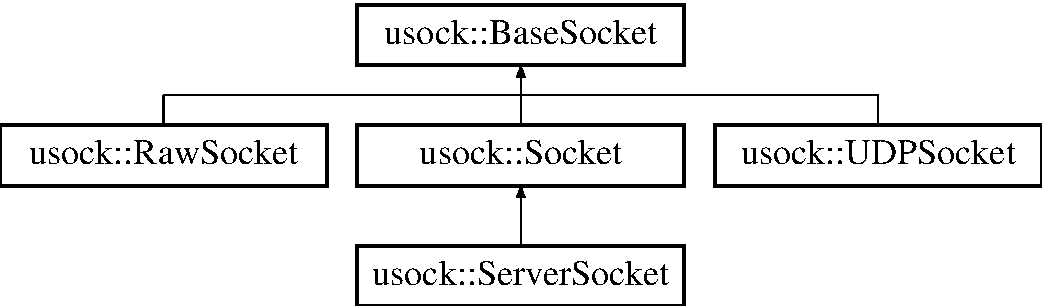
\includegraphics[height=3cm]{classusock_1_1BaseSocket}
\end{center}
\end{figure}
\subsection*{Public Types}
\begin{CompactItemize}
\item 
enum \hyperlink{classusock_1_1BaseSocket_50d8769de87937b42f8cef370917aa0b}{target} \{ \hyperlink{classusock_1_1BaseSocket_50d8769de87937b42f8cef370917aa0b13bac8e60708dc8451b1addafbd3dd77}{any} =  INADDR\_\-ANY, 
\hyperlink{classusock_1_1BaseSocket_50d8769de87937b42f8cef370917aa0b1bf59b5083e7c55e7bf86ec50291d617}{broadcat} =  INADDR\_\-BROADCAST, 
\hyperlink{classusock_1_1BaseSocket_50d8769de87937b42f8cef370917aa0bbefd2832243f347df978af6409917c38}{loopback} =  INADDR\_\-LOOPBACK, 
\hyperlink{classusock_1_1BaseSocket_50d8769de87937b42f8cef370917aa0b2e5c5b23744de44c69004e477510d95b}{none} =  INADDR\_\-NONE
 \}
\begin{CompactList}\small\item\em Enum for describing possible socket targets. \item\end{CompactList}\item 
enum \hyperlink{classusock_1_1BaseSocket_a51cae0b366638a5f697f64174135d90}{domain} \{ \hyperlink{classusock_1_1BaseSocket_a51cae0b366638a5f697f64174135d904293c75d794987e0017bab42bbbcbf73}{inet} =  AF\_\-INET, 
\hyperlink{classusock_1_1BaseSocket_a51cae0b366638a5f697f64174135d9089db67cd78ea92b1ca5bf823ca967680}{inet6} =  AF\_\-INET6
 \}
\begin{CompactList}\small\item\em Enum for describing socket domains. \item\end{CompactList}\item 
enum \hyperlink{classusock_1_1BaseSocket_8117d25c7b482eb594d68137868ce5f9}{type} \{ \par
\hyperlink{classusock_1_1BaseSocket_8117d25c7b482eb594d68137868ce5f94052647af14af3924e9b994a5ab53b8e}{sock\_\-stream} =  SOCK\_\-STREAM, 
\hyperlink{classusock_1_1BaseSocket_8117d25c7b482eb594d68137868ce5f95b0f0651f7544fbc1fedc8997d914365}{sock\_\-dgram} =  SOCK\_\-DGRAM, 
\hyperlink{classusock_1_1BaseSocket_8117d25c7b482eb594d68137868ce5f9d3b8cbf378c46eb82b5a0039eab34ca7}{sock\_\-raw} =  SOCK\_\-RAW, 
\hyperlink{classusock_1_1BaseSocket_8117d25c7b482eb594d68137868ce5f9e04a390261efe04335235f26a00b72d5}{sock\_\-rdm} =  SOCK\_\-RDM, 
\par
\hyperlink{classusock_1_1BaseSocket_8117d25c7b482eb594d68137868ce5f9adfa1bc59768fc0be580b4ba95c6f357}{sock\_\-seq} =  SOCK\_\-SEQPACKET
 \}
\begin{CompactList}\small\item\em Enum for describing socket types. \item\end{CompactList}\item 
enum \hyperlink{classusock_1_1BaseSocket_09208675b41c416fb402824742963eaa}{protocol} \{ \par
\hyperlink{classusock_1_1BaseSocket_09208675b41c416fb402824742963eaabf22c7bfd50adb88e468d3744e932497}{ip} =  IPPROTO\_\-IP, 
\hyperlink{classusock_1_1BaseSocket_09208675b41c416fb402824742963eaa3a17ad9b4036c0957dc098c76e8fba2a}{tcp} =  IPPROTO\_\-TCP, 
\hyperlink{classusock_1_1BaseSocket_09208675b41c416fb402824742963eaae0719b1eee901237a5ec0ba9031cdfce}{udp} =  IPPROTO\_\-UDP, 
\hyperlink{classusock_1_1BaseSocket_09208675b41c416fb402824742963eaa0d09509fb52df026fec01b98795f9ac4}{raw} =  IPPROTO\_\-RAW, 
\par
\hyperlink{classusock_1_1BaseSocket_09208675b41c416fb402824742963eaa5c569c4f7525d07ee96857a015d057bb}{icmp} =  IPPROTO\_\-ICMP
 \}
\begin{CompactList}\small\item\em Enum for describing socket protocols. \item\end{CompactList}\end{CompactItemize}
\subsection*{Public Member Functions}
\begin{CompactItemize}
\item 
\hyperlink{classusock_1_1BaseSocket_5cf4bfad30ea514f522101899592b97f}{BaseSocket} (int \hyperlink{classusock_1_1BaseSocket_a51cae0b366638a5f697f64174135d90}{domain}, int \hyperlink{classusock_1_1BaseSocket_8117d25c7b482eb594d68137868ce5f9}{type}, int \hyperlink{classusock_1_1BaseSocket_09208675b41c416fb402824742963eaa}{protocol}, double \hyperlink{classusock_1_1BaseSocket_b419e8fd0b849c74b73a02d6bd9081e3}{timeout}=0.0)  throw ()
\begin{CompactList}\small\item\em Constructor for the \hyperlink{classusock_1_1BaseSocket}{BaseSocket} class. \item\end{CompactList}\item 
\hyperlink{classusock_1_1BaseSocket_60ad362afb927b4d4e7233c5e9735c7b}{$\sim$BaseSocket} ()
\begin{CompactList}\small\item\em Destroyer for the \hyperlink{classusock_1_1Socket}{Socket} class (it just destroyes our socket descriptor). \item\end{CompactList}\item 
void \hyperlink{classusock_1_1BaseSocket_06383c7ad352244fb0e5e6276e5e86c2}{close} ()
\begin{CompactList}\small\item\em Close the socket descriptor. \item\end{CompactList}\item 
std::string \hyperlink{classusock_1_1BaseSocket_7ffc3a11be4a9d7ba72a1f66f3dbad68}{getHostByName} (const std::string \&name)  throw ()
\begin{CompactList}\small\item\em Wrap method around gethostbyname() function. \item\end{CompactList}\item 
std::string \hyperlink{classusock_1_1BaseSocket_b0fdf738e659b1d7088611bd4b4c9b67}{getHostByAddr} (const std::string \&addr)  throw ()
\begin{CompactList}\small\item\em Wrap method around gethostbyaddr() function. \item\end{CompactList}\item 
void \hyperlink{classusock_1_1BaseSocket_143722edec56e119495fb8ded76582e5}{setBlocking} (bool f=true)  throw ()
\begin{CompactList}\small\item\em Set or unset the blocking flag on a socket. \item\end{CompactList}\item 
bool \hyperlink{classusock_1_1BaseSocket_d29a1fabc8b4c7a86cd236473ef03177}{isBlocking} ()  throw ()
\begin{CompactList}\small\item\em Checks whether a socket is blocking. \item\end{CompactList}\item 
std::string \hyperlink{classusock_1_1BaseSocket_479da55516dcda8117a356d8a3be3d83}{localAddr} ()  throw ()
\begin{CompactList}\small\item\em Return the local address assigned to a socket descriptor. \item\end{CompactList}\item 
std::string \hyperlink{classusock_1_1BaseSocket_3842fc1ea6ac5575e988d4ee620089a7}{remoteAddr} ()  throw ()
\begin{CompactList}\small\item\em Return the remote address to which the socket is linked. \item\end{CompactList}\item 
u\_\-int16\_\-t \hyperlink{classusock_1_1BaseSocket_47218f0ff53693f2891573ec47d84f36}{localPort} ()  throw ()
\begin{CompactList}\small\item\em Return the local port. \item\end{CompactList}\item 
u\_\-int16\_\-t \hyperlink{classusock_1_1BaseSocket_e4e09d33779e097ada03144ff54286aa}{remotePort} ()  throw ()
\begin{CompactList}\small\item\em Return the remote port. \item\end{CompactList}\item 
void \hyperlink{classusock_1_1BaseSocket_87925e8c3b89a50f8c8c2a68e0d2ab70}{getSockOpt} (int level, int optname, void $\ast$optval, socklen\_\-t $\ast$optlen)  throw ()
\begin{CompactList}\small\item\em Wrap around getsockopt() function. \item\end{CompactList}\item 
void \hyperlink{classusock_1_1BaseSocket_d0444de98899e9312bfa320d5a359e07}{setSockOpt} (int level, int optname, void $\ast$optval, socklen\_\-t optlen)  throw ()
\begin{CompactList}\small\item\em Wrap around setsockopt() function. \item\end{CompactList}\item 
void \hyperlink{classusock_1_1BaseSocket_e31552b42df68bc68fe557caf6e75128}{setTimeout} (double \hyperlink{classusock_1_1BaseSocket_b419e8fd0b849c74b73a02d6bd9081e3}{timeout}=0.0)  throw ()
\begin{CompactList}\small\item\em Set a timeout (in seconds) on the socket. \item\end{CompactList}\item 
std::string \hyperlink{classusock_1_1BaseSocket_3da108b8c23df3b521ded0bc4ae5295c}{ntoa} (in\_\-addr\_\-t addr)  throw ()
\begin{CompactList}\small\item\em Wrap around inet\_\-ntoa() function, it returns an ASCII string, given a 32 bit IPv4 address. \item\end{CompactList}\end{CompactItemize}
\subsection*{Protected Member Functions}
\begin{CompactItemize}
\item 
\hyperlink{classusock_1_1BaseSocket_20f598433d6c3a97656f0179f7371218}{BaseSocket} ()
\begin{CompactList}\small\item\em Empty \hyperlink{classusock_1_1BaseSocket}{BaseSocket} constructor - ONLY used inside the children classes to initialize a \hyperlink{classusock_1_1Socket}{Socket} object using an already existen socket descriptor. \item\end{CompactList}\end{CompactItemize}
\subsection*{Protected Attributes}
\begin{CompactItemize}
\item 
int \hyperlink{classusock_1_1BaseSocket_63b6c07fb14f937056148cbf8b3531c5}{sd}
\begin{CompactList}\small\item\em Private socket descriptor. \item\end{CompactList}\item 
int \hyperlink{classusock_1_1BaseSocket_9a7414d934aeccd1340292214a2aef0e}{domain}
\begin{CompactList}\small\item\em Domain for the socket. \item\end{CompactList}\item 
int \hyperlink{classusock_1_1BaseSocket_139a74d163977332762f349a73f4bd64}{type}
\begin{CompactList}\small\item\em \hyperlink{classusock_1_1Socket}{Socket} type. \item\end{CompactList}\item 
int \hyperlink{classusock_1_1BaseSocket_91b9f72f183b6314891f7e1f93ead99a}{protocol}
\begin{CompactList}\small\item\em \hyperlink{classusock_1_1Socket}{Socket} protocol. \item\end{CompactList}\item 
double \hyperlink{classusock_1_1BaseSocket_b419e8fd0b849c74b73a02d6bd9081e3}{timeout}
\begin{CompactList}\small\item\em Optional timeout for connect/send/receive operations (default: no timeout, timeout = 0.0). \item\end{CompactList}\end{CompactItemize}


\subsection{Detailed Description}
Class for describing basic sockets. 

\begin{Desc}
\item[Author:]BlackLight \end{Desc}


\subsection{Member Enumeration Documentation}
\hypertarget{classusock_1_1BaseSocket_a51cae0b366638a5f697f64174135d90}{
\index{usock::BaseSocket@{usock::BaseSocket}!domain@{domain}}
\index{domain@{domain}!usock::BaseSocket@{usock::BaseSocket}}
\subsubsection[{domain}]{\setlength{\rightskip}{0pt plus 5cm}enum {\bf usock::BaseSocket::domain}}}
\label{classusock_1_1BaseSocket_a51cae0b366638a5f697f64174135d90}


Enum for describing socket domains. 

\begin{Desc}
\item[Enumerator: ]\par
\begin{description}
\index{inet@{inet}!usock::BaseSocket@{usock::BaseSocket}}\index{usock::BaseSocket@{usock::BaseSocket}!inet@{inet}}\item[{\em 
\hypertarget{classusock_1_1BaseSocket_a51cae0b366638a5f697f64174135d904293c75d794987e0017bab42bbbcbf73}{
inet}
\label{classusock_1_1BaseSocket_a51cae0b366638a5f697f64174135d904293c75d794987e0017bab42bbbcbf73}
}]\index{inet6@{inet6}!usock::BaseSocket@{usock::BaseSocket}}\index{usock::BaseSocket@{usock::BaseSocket}!inet6@{inet6}}\item[{\em 
\hypertarget{classusock_1_1BaseSocket_a51cae0b366638a5f697f64174135d9089db67cd78ea92b1ca5bf823ca967680}{
inet6}
\label{classusock_1_1BaseSocket_a51cae0b366638a5f697f64174135d9089db67cd78ea92b1ca5bf823ca967680}
}]\end{description}
\end{Desc}

\hypertarget{classusock_1_1BaseSocket_09208675b41c416fb402824742963eaa}{
\index{usock::BaseSocket@{usock::BaseSocket}!protocol@{protocol}}
\index{protocol@{protocol}!usock::BaseSocket@{usock::BaseSocket}}
\subsubsection[{protocol}]{\setlength{\rightskip}{0pt plus 5cm}enum {\bf usock::BaseSocket::protocol}}}
\label{classusock_1_1BaseSocket_09208675b41c416fb402824742963eaa}


Enum for describing socket protocols. 

\begin{Desc}
\item[Enumerator: ]\par
\begin{description}
\index{ip@{ip}!usock::BaseSocket@{usock::BaseSocket}}\index{usock::BaseSocket@{usock::BaseSocket}!ip@{ip}}\item[{\em 
\hypertarget{classusock_1_1BaseSocket_09208675b41c416fb402824742963eaabf22c7bfd50adb88e468d3744e932497}{
ip}
\label{classusock_1_1BaseSocket_09208675b41c416fb402824742963eaabf22c7bfd50adb88e468d3744e932497}
}]\index{tcp@{tcp}!usock::BaseSocket@{usock::BaseSocket}}\index{usock::BaseSocket@{usock::BaseSocket}!tcp@{tcp}}\item[{\em 
\hypertarget{classusock_1_1BaseSocket_09208675b41c416fb402824742963eaa3a17ad9b4036c0957dc098c76e8fba2a}{
tcp}
\label{classusock_1_1BaseSocket_09208675b41c416fb402824742963eaa3a17ad9b4036c0957dc098c76e8fba2a}
}]\index{udp@{udp}!usock::BaseSocket@{usock::BaseSocket}}\index{usock::BaseSocket@{usock::BaseSocket}!udp@{udp}}\item[{\em 
\hypertarget{classusock_1_1BaseSocket_09208675b41c416fb402824742963eaae0719b1eee901237a5ec0ba9031cdfce}{
udp}
\label{classusock_1_1BaseSocket_09208675b41c416fb402824742963eaae0719b1eee901237a5ec0ba9031cdfce}
}]\index{raw@{raw}!usock::BaseSocket@{usock::BaseSocket}}\index{usock::BaseSocket@{usock::BaseSocket}!raw@{raw}}\item[{\em 
\hypertarget{classusock_1_1BaseSocket_09208675b41c416fb402824742963eaa0d09509fb52df026fec01b98795f9ac4}{
raw}
\label{classusock_1_1BaseSocket_09208675b41c416fb402824742963eaa0d09509fb52df026fec01b98795f9ac4}
}]\index{icmp@{icmp}!usock::BaseSocket@{usock::BaseSocket}}\index{usock::BaseSocket@{usock::BaseSocket}!icmp@{icmp}}\item[{\em 
\hypertarget{classusock_1_1BaseSocket_09208675b41c416fb402824742963eaa5c569c4f7525d07ee96857a015d057bb}{
icmp}
\label{classusock_1_1BaseSocket_09208675b41c416fb402824742963eaa5c569c4f7525d07ee96857a015d057bb}
}]\end{description}
\end{Desc}

\hypertarget{classusock_1_1BaseSocket_50d8769de87937b42f8cef370917aa0b}{
\index{usock::BaseSocket@{usock::BaseSocket}!target@{target}}
\index{target@{target}!usock::BaseSocket@{usock::BaseSocket}}
\subsubsection[{target}]{\setlength{\rightskip}{0pt plus 5cm}enum {\bf usock::BaseSocket::target}}}
\label{classusock_1_1BaseSocket_50d8769de87937b42f8cef370917aa0b}


Enum for describing possible socket targets. 

\begin{Desc}
\item[Enumerator: ]\par
\begin{description}
\index{any@{any}!usock::BaseSocket@{usock::BaseSocket}}\index{usock::BaseSocket@{usock::BaseSocket}!any@{any}}\item[{\em 
\hypertarget{classusock_1_1BaseSocket_50d8769de87937b42f8cef370917aa0b13bac8e60708dc8451b1addafbd3dd77}{
any}
\label{classusock_1_1BaseSocket_50d8769de87937b42f8cef370917aa0b13bac8e60708dc8451b1addafbd3dd77}
}]\index{broadcat@{broadcat}!usock::BaseSocket@{usock::BaseSocket}}\index{usock::BaseSocket@{usock::BaseSocket}!broadcat@{broadcat}}\item[{\em 
\hypertarget{classusock_1_1BaseSocket_50d8769de87937b42f8cef370917aa0b1bf59b5083e7c55e7bf86ec50291d617}{
broadcat}
\label{classusock_1_1BaseSocket_50d8769de87937b42f8cef370917aa0b1bf59b5083e7c55e7bf86ec50291d617}
}]\index{loopback@{loopback}!usock::BaseSocket@{usock::BaseSocket}}\index{usock::BaseSocket@{usock::BaseSocket}!loopback@{loopback}}\item[{\em 
\hypertarget{classusock_1_1BaseSocket_50d8769de87937b42f8cef370917aa0bbefd2832243f347df978af6409917c38}{
loopback}
\label{classusock_1_1BaseSocket_50d8769de87937b42f8cef370917aa0bbefd2832243f347df978af6409917c38}
}]\index{none@{none}!usock::BaseSocket@{usock::BaseSocket}}\index{usock::BaseSocket@{usock::BaseSocket}!none@{none}}\item[{\em 
\hypertarget{classusock_1_1BaseSocket_50d8769de87937b42f8cef370917aa0b2e5c5b23744de44c69004e477510d95b}{
none}
\label{classusock_1_1BaseSocket_50d8769de87937b42f8cef370917aa0b2e5c5b23744de44c69004e477510d95b}
}]\end{description}
\end{Desc}

\hypertarget{classusock_1_1BaseSocket_8117d25c7b482eb594d68137868ce5f9}{
\index{usock::BaseSocket@{usock::BaseSocket}!type@{type}}
\index{type@{type}!usock::BaseSocket@{usock::BaseSocket}}
\subsubsection[{type}]{\setlength{\rightskip}{0pt plus 5cm}enum {\bf usock::BaseSocket::type}}}
\label{classusock_1_1BaseSocket_8117d25c7b482eb594d68137868ce5f9}


Enum for describing socket types. 

\begin{Desc}
\item[Enumerator: ]\par
\begin{description}
\index{sock\_\-stream@{sock\_\-stream}!usock::BaseSocket@{usock::BaseSocket}}\index{usock::BaseSocket@{usock::BaseSocket}!sock\_\-stream@{sock\_\-stream}}\item[{\em 
\hypertarget{classusock_1_1BaseSocket_8117d25c7b482eb594d68137868ce5f94052647af14af3924e9b994a5ab53b8e}{
sock\_\-stream}
\label{classusock_1_1BaseSocket_8117d25c7b482eb594d68137868ce5f94052647af14af3924e9b994a5ab53b8e}
}]\index{sock\_\-dgram@{sock\_\-dgram}!usock::BaseSocket@{usock::BaseSocket}}\index{usock::BaseSocket@{usock::BaseSocket}!sock\_\-dgram@{sock\_\-dgram}}\item[{\em 
\hypertarget{classusock_1_1BaseSocket_8117d25c7b482eb594d68137868ce5f95b0f0651f7544fbc1fedc8997d914365}{
sock\_\-dgram}
\label{classusock_1_1BaseSocket_8117d25c7b482eb594d68137868ce5f95b0f0651f7544fbc1fedc8997d914365}
}]\index{sock\_\-raw@{sock\_\-raw}!usock::BaseSocket@{usock::BaseSocket}}\index{usock::BaseSocket@{usock::BaseSocket}!sock\_\-raw@{sock\_\-raw}}\item[{\em 
\hypertarget{classusock_1_1BaseSocket_8117d25c7b482eb594d68137868ce5f9d3b8cbf378c46eb82b5a0039eab34ca7}{
sock\_\-raw}
\label{classusock_1_1BaseSocket_8117d25c7b482eb594d68137868ce5f9d3b8cbf378c46eb82b5a0039eab34ca7}
}]\index{sock\_\-rdm@{sock\_\-rdm}!usock::BaseSocket@{usock::BaseSocket}}\index{usock::BaseSocket@{usock::BaseSocket}!sock\_\-rdm@{sock\_\-rdm}}\item[{\em 
\hypertarget{classusock_1_1BaseSocket_8117d25c7b482eb594d68137868ce5f9e04a390261efe04335235f26a00b72d5}{
sock\_\-rdm}
\label{classusock_1_1BaseSocket_8117d25c7b482eb594d68137868ce5f9e04a390261efe04335235f26a00b72d5}
}]\index{sock\_\-seq@{sock\_\-seq}!usock::BaseSocket@{usock::BaseSocket}}\index{usock::BaseSocket@{usock::BaseSocket}!sock\_\-seq@{sock\_\-seq}}\item[{\em 
\hypertarget{classusock_1_1BaseSocket_8117d25c7b482eb594d68137868ce5f9adfa1bc59768fc0be580b4ba95c6f357}{
sock\_\-seq}
\label{classusock_1_1BaseSocket_8117d25c7b482eb594d68137868ce5f9adfa1bc59768fc0be580b4ba95c6f357}
}]\end{description}
\end{Desc}



\subsection{Constructor \& Destructor Documentation}
\hypertarget{classusock_1_1BaseSocket_20f598433d6c3a97656f0179f7371218}{
\index{usock::BaseSocket@{usock::BaseSocket}!BaseSocket@{BaseSocket}}
\index{BaseSocket@{BaseSocket}!usock::BaseSocket@{usock::BaseSocket}}
\subsubsection[{BaseSocket}]{\setlength{\rightskip}{0pt plus 5cm}usock::BaseSocket::BaseSocket ()\hspace{0.3cm}{\tt  \mbox{[}inline, protected\mbox{]}}}}
\label{classusock_1_1BaseSocket_20f598433d6c3a97656f0179f7371218}


Empty \hyperlink{classusock_1_1BaseSocket}{BaseSocket} constructor - ONLY used inside the children classes to initialize a \hyperlink{classusock_1_1Socket}{Socket} object using an already existen socket descriptor. 

\hypertarget{classusock_1_1BaseSocket_5cf4bfad30ea514f522101899592b97f}{
\index{usock::BaseSocket@{usock::BaseSocket}!BaseSocket@{BaseSocket}}
\index{BaseSocket@{BaseSocket}!usock::BaseSocket@{usock::BaseSocket}}
\subsubsection[{BaseSocket}]{\setlength{\rightskip}{0pt plus 5cm}usock::BaseSocket::BaseSocket (int {\em domain}, \/  int {\em type}, \/  int {\em protocol}, \/  double {\em timeout} = {\tt 0.0})  throw ()}}
\label{classusock_1_1BaseSocket_5cf4bfad30ea514f522101899592b97f}


Constructor for the \hyperlink{classusock_1_1BaseSocket}{BaseSocket} class. 

\begin{Desc}
\item[Parameters:]
\begin{description}
\item[{\em domain}]\hyperlink{classusock_1_1Socket}{Socket} domain \item[{\em type}]\hyperlink{classusock_1_1Socket}{Socket} type \item[{\em protocol}]\hyperlink{classusock_1_1Socket}{Socket} protocol \item[{\em timeout}]\hyperlink{classusock_1_1Socket}{Socket} timeout for send/recv/connect operations \end{description}
\end{Desc}
\hypertarget{classusock_1_1BaseSocket_60ad362afb927b4d4e7233c5e9735c7b}{
\index{usock::BaseSocket@{usock::BaseSocket}!$\sim$BaseSocket@{$\sim$BaseSocket}}
\index{$\sim$BaseSocket@{$\sim$BaseSocket}!usock::BaseSocket@{usock::BaseSocket}}
\subsubsection[{$\sim$BaseSocket}]{\setlength{\rightskip}{0pt plus 5cm}usock::BaseSocket::$\sim$BaseSocket ()}}
\label{classusock_1_1BaseSocket_60ad362afb927b4d4e7233c5e9735c7b}


Destroyer for the \hyperlink{classusock_1_1Socket}{Socket} class (it just destroyes our socket descriptor). 



\subsection{Member Function Documentation}
\hypertarget{classusock_1_1BaseSocket_06383c7ad352244fb0e5e6276e5e86c2}{
\index{usock::BaseSocket@{usock::BaseSocket}!close@{close}}
\index{close@{close}!usock::BaseSocket@{usock::BaseSocket}}
\subsubsection[{close}]{\setlength{\rightskip}{0pt plus 5cm}void usock::BaseSocket::close ()}}
\label{classusock_1_1BaseSocket_06383c7ad352244fb0e5e6276e5e86c2}


Close the socket descriptor. 

\hypertarget{classusock_1_1BaseSocket_b0fdf738e659b1d7088611bd4b4c9b67}{
\index{usock::BaseSocket@{usock::BaseSocket}!getHostByAddr@{getHostByAddr}}
\index{getHostByAddr@{getHostByAddr}!usock::BaseSocket@{usock::BaseSocket}}
\subsubsection[{getHostByAddr}]{\setlength{\rightskip}{0pt plus 5cm}std::string usock::BaseSocket::getHostByAddr (const std::string \& {\em addr})  throw ()}}
\label{classusock_1_1BaseSocket_b0fdf738e659b1d7088611bd4b4c9b67}


Wrap method around gethostbyaddr() function. 

\begin{Desc}
\item[Parameters:]
\begin{description}
\item[{\em addr}]IPv4 address as a string \end{description}
\end{Desc}
\begin{Desc}
\item[Returns:]The hostname associated to addr, if found, an empty otherwise \end{Desc}
\hypertarget{classusock_1_1BaseSocket_7ffc3a11be4a9d7ba72a1f66f3dbad68}{
\index{usock::BaseSocket@{usock::BaseSocket}!getHostByName@{getHostByName}}
\index{getHostByName@{getHostByName}!usock::BaseSocket@{usock::BaseSocket}}
\subsubsection[{getHostByName}]{\setlength{\rightskip}{0pt plus 5cm}std::string usock::BaseSocket::getHostByName (const std::string \& {\em name})  throw ()}}
\label{classusock_1_1BaseSocket_7ffc3a11be4a9d7ba72a1f66f3dbad68}


Wrap method around gethostbyname() function. 

\begin{Desc}
\item[Parameters:]
\begin{description}
\item[{\em name}]Host name \end{description}
\end{Desc}
\begin{Desc}
\item[Returns:]IP address of our host name, if found, an empty string otherwise \end{Desc}
\hypertarget{classusock_1_1BaseSocket_87925e8c3b89a50f8c8c2a68e0d2ab70}{
\index{usock::BaseSocket@{usock::BaseSocket}!getSockOpt@{getSockOpt}}
\index{getSockOpt@{getSockOpt}!usock::BaseSocket@{usock::BaseSocket}}
\subsubsection[{getSockOpt}]{\setlength{\rightskip}{0pt plus 5cm}void usock::BaseSocket::getSockOpt (int {\em level}, \/  int {\em optname}, \/  void $\ast$ {\em optval}, \/  socklen\_\-t $\ast$ {\em optlen})  throw ()}}
\label{classusock_1_1BaseSocket_87925e8c3b89a50f8c8c2a68e0d2ab70}


Wrap around getsockopt() function. 

\hypertarget{classusock_1_1BaseSocket_d29a1fabc8b4c7a86cd236473ef03177}{
\index{usock::BaseSocket@{usock::BaseSocket}!isBlocking@{isBlocking}}
\index{isBlocking@{isBlocking}!usock::BaseSocket@{usock::BaseSocket}}
\subsubsection[{isBlocking}]{\setlength{\rightskip}{0pt plus 5cm}bool usock::BaseSocket::isBlocking ()  throw ()}}
\label{classusock_1_1BaseSocket_d29a1fabc8b4c7a86cd236473ef03177}


Checks whether a socket is blocking. 

\begin{Desc}
\item[Returns:]true if the socket is blocking, false otherwise \end{Desc}
\hypertarget{classusock_1_1BaseSocket_479da55516dcda8117a356d8a3be3d83}{
\index{usock::BaseSocket@{usock::BaseSocket}!localAddr@{localAddr}}
\index{localAddr@{localAddr}!usock::BaseSocket@{usock::BaseSocket}}
\subsubsection[{localAddr}]{\setlength{\rightskip}{0pt plus 5cm}std::string usock::BaseSocket::localAddr ()  throw ()}}
\label{classusock_1_1BaseSocket_479da55516dcda8117a356d8a3be3d83}


Return the local address assigned to a socket descriptor. 

\hypertarget{classusock_1_1BaseSocket_47218f0ff53693f2891573ec47d84f36}{
\index{usock::BaseSocket@{usock::BaseSocket}!localPort@{localPort}}
\index{localPort@{localPort}!usock::BaseSocket@{usock::BaseSocket}}
\subsubsection[{localPort}]{\setlength{\rightskip}{0pt plus 5cm}u\_\-int16\_\-t usock::BaseSocket::localPort ()  throw ()}}
\label{classusock_1_1BaseSocket_47218f0ff53693f2891573ec47d84f36}


Return the local port. 

\hypertarget{classusock_1_1BaseSocket_3da108b8c23df3b521ded0bc4ae5295c}{
\index{usock::BaseSocket@{usock::BaseSocket}!ntoa@{ntoa}}
\index{ntoa@{ntoa}!usock::BaseSocket@{usock::BaseSocket}}
\subsubsection[{ntoa}]{\setlength{\rightskip}{0pt plus 5cm}std::string usock::BaseSocket::ntoa (in\_\-addr\_\-t {\em addr})  throw ()}}
\label{classusock_1_1BaseSocket_3da108b8c23df3b521ded0bc4ae5295c}


Wrap around inet\_\-ntoa() function, it returns an ASCII string, given a 32 bit IPv4 address. 

\begin{Desc}
\item[Parameters:]
\begin{description}
\item[{\em addr}]IPv4 32 bit address \end{description}
\end{Desc}
\hypertarget{classusock_1_1BaseSocket_3842fc1ea6ac5575e988d4ee620089a7}{
\index{usock::BaseSocket@{usock::BaseSocket}!remoteAddr@{remoteAddr}}
\index{remoteAddr@{remoteAddr}!usock::BaseSocket@{usock::BaseSocket}}
\subsubsection[{remoteAddr}]{\setlength{\rightskip}{0pt plus 5cm}std::string usock::BaseSocket::remoteAddr ()  throw ()}}
\label{classusock_1_1BaseSocket_3842fc1ea6ac5575e988d4ee620089a7}


Return the remote address to which the socket is linked. 

\hypertarget{classusock_1_1BaseSocket_e4e09d33779e097ada03144ff54286aa}{
\index{usock::BaseSocket@{usock::BaseSocket}!remotePort@{remotePort}}
\index{remotePort@{remotePort}!usock::BaseSocket@{usock::BaseSocket}}
\subsubsection[{remotePort}]{\setlength{\rightskip}{0pt plus 5cm}u\_\-int16\_\-t usock::BaseSocket::remotePort ()  throw ()}}
\label{classusock_1_1BaseSocket_e4e09d33779e097ada03144ff54286aa}


Return the remote port. 

\hypertarget{classusock_1_1BaseSocket_143722edec56e119495fb8ded76582e5}{
\index{usock::BaseSocket@{usock::BaseSocket}!setBlocking@{setBlocking}}
\index{setBlocking@{setBlocking}!usock::BaseSocket@{usock::BaseSocket}}
\subsubsection[{setBlocking}]{\setlength{\rightskip}{0pt plus 5cm}void usock::BaseSocket::setBlocking (bool {\em f} = {\tt true})  throw ()}}
\label{classusock_1_1BaseSocket_143722edec56e119495fb8ded76582e5}


Set or unset the blocking flag on a socket. 

\begin{Desc}
\item[Parameters:]
\begin{description}
\item[{\em f}]Boolean flag (true/false) \end{description}
\end{Desc}
\hypertarget{classusock_1_1BaseSocket_d0444de98899e9312bfa320d5a359e07}{
\index{usock::BaseSocket@{usock::BaseSocket}!setSockOpt@{setSockOpt}}
\index{setSockOpt@{setSockOpt}!usock::BaseSocket@{usock::BaseSocket}}
\subsubsection[{setSockOpt}]{\setlength{\rightskip}{0pt plus 5cm}void usock::BaseSocket::setSockOpt (int {\em level}, \/  int {\em optname}, \/  void $\ast$ {\em optval}, \/  socklen\_\-t {\em optlen})  throw ()}}
\label{classusock_1_1BaseSocket_d0444de98899e9312bfa320d5a359e07}


Wrap around setsockopt() function. 

\hypertarget{classusock_1_1BaseSocket_e31552b42df68bc68fe557caf6e75128}{
\index{usock::BaseSocket@{usock::BaseSocket}!setTimeout@{setTimeout}}
\index{setTimeout@{setTimeout}!usock::BaseSocket@{usock::BaseSocket}}
\subsubsection[{setTimeout}]{\setlength{\rightskip}{0pt plus 5cm}void usock::BaseSocket::setTimeout (double {\em timeout} = {\tt 0.0})  throw ()}}
\label{classusock_1_1BaseSocket_e31552b42df68bc68fe557caf6e75128}


Set a timeout (in seconds) on the socket. 

\begin{Desc}
\item[Parameters:]
\begin{description}
\item[{\em timeout}]Second we're going to wait. It's a double value, so you can specify decimal digits to have a granularity precision bigger than the seconds \end{description}
\end{Desc}


\subsection{Member Data Documentation}
\hypertarget{classusock_1_1BaseSocket_9a7414d934aeccd1340292214a2aef0e}{
\index{usock::BaseSocket@{usock::BaseSocket}!domain@{domain}}
\index{domain@{domain}!usock::BaseSocket@{usock::BaseSocket}}
\subsubsection[{domain}]{\setlength{\rightskip}{0pt plus 5cm}int {\bf usock::BaseSocket::domain}\hspace{0.3cm}{\tt  \mbox{[}protected\mbox{]}}}}
\label{classusock_1_1BaseSocket_9a7414d934aeccd1340292214a2aef0e}


Domain for the socket. 

\hypertarget{classusock_1_1BaseSocket_91b9f72f183b6314891f7e1f93ead99a}{
\index{usock::BaseSocket@{usock::BaseSocket}!protocol@{protocol}}
\index{protocol@{protocol}!usock::BaseSocket@{usock::BaseSocket}}
\subsubsection[{protocol}]{\setlength{\rightskip}{0pt plus 5cm}int {\bf usock::BaseSocket::protocol}\hspace{0.3cm}{\tt  \mbox{[}protected\mbox{]}}}}
\label{classusock_1_1BaseSocket_91b9f72f183b6314891f7e1f93ead99a}


\hyperlink{classusock_1_1Socket}{Socket} protocol. 

\hypertarget{classusock_1_1BaseSocket_63b6c07fb14f937056148cbf8b3531c5}{
\index{usock::BaseSocket@{usock::BaseSocket}!sd@{sd}}
\index{sd@{sd}!usock::BaseSocket@{usock::BaseSocket}}
\subsubsection[{sd}]{\setlength{\rightskip}{0pt plus 5cm}int {\bf usock::BaseSocket::sd}\hspace{0.3cm}{\tt  \mbox{[}protected\mbox{]}}}}
\label{classusock_1_1BaseSocket_63b6c07fb14f937056148cbf8b3531c5}


Private socket descriptor. 

\hypertarget{classusock_1_1BaseSocket_b419e8fd0b849c74b73a02d6bd9081e3}{
\index{usock::BaseSocket@{usock::BaseSocket}!timeout@{timeout}}
\index{timeout@{timeout}!usock::BaseSocket@{usock::BaseSocket}}
\subsubsection[{timeout}]{\setlength{\rightskip}{0pt plus 5cm}double {\bf usock::BaseSocket::timeout}\hspace{0.3cm}{\tt  \mbox{[}protected\mbox{]}}}}
\label{classusock_1_1BaseSocket_b419e8fd0b849c74b73a02d6bd9081e3}


Optional timeout for connect/send/receive operations (default: no timeout, timeout = 0.0). 

\hypertarget{classusock_1_1BaseSocket_139a74d163977332762f349a73f4bd64}{
\index{usock::BaseSocket@{usock::BaseSocket}!type@{type}}
\index{type@{type}!usock::BaseSocket@{usock::BaseSocket}}
\subsubsection[{type}]{\setlength{\rightskip}{0pt plus 5cm}int {\bf usock::BaseSocket::type}\hspace{0.3cm}{\tt  \mbox{[}protected\mbox{]}}}}
\label{classusock_1_1BaseSocket_139a74d163977332762f349a73f4bd64}


\hyperlink{classusock_1_1Socket}{Socket} type. 



The documentation for this class was generated from the following file:\begin{CompactItemize}
\item 
\hyperlink{usock_8h}{usock.h}\end{CompactItemize}

\hypertarget{classusock_1_1RawSocket}{
\section{usock::RawSocket Class Reference}
\label{classusock_1_1RawSocket}\index{usock::RawSocket@{usock::RawSocket}}
}
Class for managing raw sockets.  


{\tt \#include $<$usock.h$>$}

Inheritance diagram for usock::RawSocket::\begin{figure}[H]
\begin{center}
\leavevmode
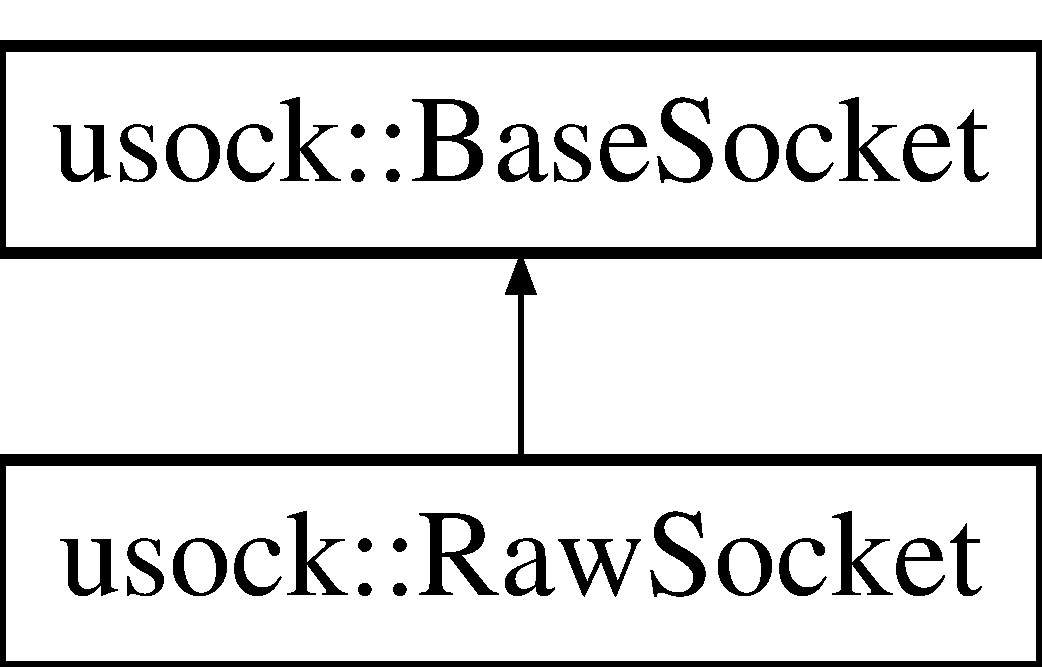
\includegraphics[height=2cm]{classusock_1_1RawSocket}
\end{center}
\end{figure}
\subsection*{Public Member Functions}
\begin{CompactItemize}
\item 
\hyperlink{classusock_1_1RawSocket_d476598f4a6db6d3cf28673172eb1b8b}{RawSocket} (std::string i=\char`\"{}lo\char`\"{})
\begin{CompactList}\small\item\em \hyperlink{classusock_1_1RawSocket}{RawSocket} constructor. \item\end{CompactList}\item 
std::string \hyperlink{classusock_1_1RawSocket_3b0c8f2f539982c8f37a66ebc29746a0}{getIPv4addr} ()  throw ()
\begin{CompactList}\small\item\em Get the IPv4 address associated to the network interface. \item\end{CompactList}\item 
std::string \hyperlink{classusock_1_1RawSocket_1276f5fcc7bc3b41d9d11055887ab7a9}{getHWaddr} ()  throw ()
\begin{CompactList}\small\item\em Get the HW address associated to the network interface. \item\end{CompactList}\item 
u\_\-int16\_\-t \hyperlink{classusock_1_1RawSocket_11c89cceced7302fe25163fbc74a6b83}{csum} (u\_\-int16\_\-t $\ast$buf, int nwords)
\begin{CompactList}\small\item\em Compute the checksum of a buffer. \item\end{CompactList}\item 
void \hyperlink{classusock_1_1RawSocket_999a433a049b33006ab8c26a7d0875b9}{buildIPv4} (std::string dst, std::string src=\char`\"{}\char`\"{}, u\_\-int8\_\-t proto=IPPROTO\_\-TCP, u\_\-int16\_\-t len=0, u\_\-int8\_\-t ttl=32, u\_\-int8\_\-t tos=0, u\_\-int16\_\-t id=0, u\_\-int16\_\-t frag=0, u\_\-int16\_\-t sum=0)
\begin{CompactList}\small\item\em Build an IPv4 header for the raw socket. \item\end{CompactList}\item 
void \hyperlink{classusock_1_1RawSocket_687afa2e3259ce2bc2cea7cc49db7f14}{buildTCP} (u\_\-int16\_\-t sport, u\_\-int16\_\-t dport, u\_\-int8\_\-t flags, u\_\-int32\_\-t seq=0, u\_\-int32\_\-t ack=0, u\_\-int16\_\-t window=0x1000, u\_\-int16\_\-t urgent=0, u\_\-int16\_\-t sum=0)
\begin{CompactList}\small\item\em Build a TCP header for the raw socket. \item\end{CompactList}\item 
void \hyperlink{classusock_1_1RawSocket_20dc8f4e7c0f5d499517b6410c5dca52}{buildUDP} (u\_\-int16\_\-t sport, u\_\-int16\_\-t dport, u\_\-int16\_\-t len=0, u\_\-int16\_\-t sum=0)
\begin{CompactList}\small\item\em Build an UDP header for the raw socket. \item\end{CompactList}\item 
void \hyperlink{classusock_1_1RawSocket_bf253d275f07db49c00f4b0d8fcf0947}{buildICMPv4} (u\_\-int8\_\-t \hyperlink{classusock_1_1BaseSocket_8117d25c7b482eb594d68137868ce5f9}{type}, u\_\-int16\_\-t id=0x100, u\_\-int16\_\-t seq=0x100, u\_\-int8\_\-t code=0, u\_\-int16\_\-t sum=0)
\begin{CompactList}\small\item\em Build an ICMPv4 header for the raw socket. \item\end{CompactList}\item 
void \hyperlink{classusock_1_1RawSocket_de9254ad3499aebabedad9b861c21bdb}{setPayload} (void $\ast$payload, int length)
\begin{CompactList}\small\item\em Set a binary payload for the raw socket. \item\end{CompactList}\item 
void \hyperlink{classusock_1_1RawSocket_ab429ec3a150c6e15175b3223c90ade6}{setPayload} (std::string payload)
\begin{CompactList}\small\item\em Set a payload for the raw socket as a string. \item\end{CompactList}\item 
void \hyperlink{classusock_1_1RawSocket_e62377b0933a176570f226e1acbe3e16}{write} ()  throw ()
\begin{CompactList}\small\item\em Write the raw packet onto the network interface. \item\end{CompactList}\item 
void $\ast$ \hyperlink{classusock_1_1RawSocket_bc4cd4449b47d28397fc270447405609}{read} (u\_\-int32\_\-t len, const std::string \&host=\char`\"{}\char`\"{})  throw ()
\begin{CompactList}\small\item\em Read binary data from the raw socket. \item\end{CompactList}\end{CompactItemize}


\subsection{Detailed Description}
Class for managing raw sockets. 

\begin{Desc}
\item[Author:]BlackLight \end{Desc}


\subsection{Constructor \& Destructor Documentation}
\hypertarget{classusock_1_1RawSocket_d476598f4a6db6d3cf28673172eb1b8b}{
\index{usock::RawSocket@{usock::RawSocket}!RawSocket@{RawSocket}}
\index{RawSocket@{RawSocket}!usock::RawSocket@{usock::RawSocket}}
\subsubsection[{RawSocket}]{\setlength{\rightskip}{0pt plus 5cm}usock::RawSocket::RawSocket (std::string {\em i} = {\tt \char`\"{}lo\char`\"{}})}}
\label{classusock_1_1RawSocket_d476598f4a6db6d3cf28673172eb1b8b}


\hyperlink{classusock_1_1RawSocket}{RawSocket} constructor. 

\begin{Desc}
\item[Parameters:]
\begin{description}
\item[{\em i}]Interface on which we're going to bind our raw socket \end{description}
\end{Desc}


\subsection{Member Function Documentation}
\hypertarget{classusock_1_1RawSocket_bf253d275f07db49c00f4b0d8fcf0947}{
\index{usock::RawSocket@{usock::RawSocket}!buildICMPv4@{buildICMPv4}}
\index{buildICMPv4@{buildICMPv4}!usock::RawSocket@{usock::RawSocket}}
\subsubsection[{buildICMPv4}]{\setlength{\rightskip}{0pt plus 5cm}void usock::RawSocket::buildICMPv4 (u\_\-int8\_\-t {\em type}, \/  u\_\-int16\_\-t {\em id} = {\tt 0x100}, \/  u\_\-int16\_\-t {\em seq} = {\tt 0x100}, \/  u\_\-int8\_\-t {\em code} = {\tt 0}, \/  u\_\-int16\_\-t {\em sum} = {\tt 0})}}
\label{classusock_1_1RawSocket_bf253d275f07db49c00f4b0d8fcf0947}


Build an ICMPv4 header for the raw socket. 

\begin{Desc}
\item[Parameters:]
\begin{description}
\item[{\em type}]ICMP type \item[{\em id}]Packet ID (default: 0x100) \item[{\em seq}]Sequence number (default: 0x100) \item[{\em code}]ICMP code (default: 0) \item[{\em sum}]ICMP checksum (default: auto-computed) \end{description}
\end{Desc}
\hypertarget{classusock_1_1RawSocket_999a433a049b33006ab8c26a7d0875b9}{
\index{usock::RawSocket@{usock::RawSocket}!buildIPv4@{buildIPv4}}
\index{buildIPv4@{buildIPv4}!usock::RawSocket@{usock::RawSocket}}
\subsubsection[{buildIPv4}]{\setlength{\rightskip}{0pt plus 5cm}void usock::RawSocket::buildIPv4 (std::string {\em dst}, \/  std::string {\em src} = {\tt \char`\"{}\char`\"{}}, \/  u\_\-int8\_\-t {\em proto} = {\tt IPPROTO\_\-TCP}, \/  u\_\-int16\_\-t {\em len} = {\tt 0}, \/  u\_\-int8\_\-t {\em ttl} = {\tt 32}, \/  u\_\-int8\_\-t {\em tos} = {\tt 0}, \/  u\_\-int16\_\-t {\em id} = {\tt 0}, \/  u\_\-int16\_\-t {\em frag} = {\tt 0}, \/  u\_\-int16\_\-t {\em sum} = {\tt 0})}}
\label{classusock_1_1RawSocket_999a433a049b33006ab8c26a7d0875b9}


Build an IPv4 header for the raw socket. 

\begin{Desc}
\item[Parameters:]
\begin{description}
\item[{\em dst}]Destination hostname/address \item[{\em src}]Source hostname/address (default: IPv4 address associated to the network interface) \item[{\em proto}]Transport protocol (default: TCP) \item[{\em len}]Total length of the IPv4 datagram (default: header length + payload length) \item[{\em ttl}]Time To Live (default: 32) \item[{\em tos}]Type Of Service (default: 0) \item[{\em id}]Datagram ID (default: 0) \item[{\em frag}]Fragmentation flag (default: 0) \item[{\em sum}]IPv4 checksum (default: auto-computed) \end{description}
\end{Desc}
\hypertarget{classusock_1_1RawSocket_687afa2e3259ce2bc2cea7cc49db7f14}{
\index{usock::RawSocket@{usock::RawSocket}!buildTCP@{buildTCP}}
\index{buildTCP@{buildTCP}!usock::RawSocket@{usock::RawSocket}}
\subsubsection[{buildTCP}]{\setlength{\rightskip}{0pt plus 5cm}void usock::RawSocket::buildTCP (u\_\-int16\_\-t {\em sport}, \/  u\_\-int16\_\-t {\em dport}, \/  u\_\-int8\_\-t {\em flags}, \/  u\_\-int32\_\-t {\em seq} = {\tt 0}, \/  u\_\-int32\_\-t {\em ack} = {\tt 0}, \/  u\_\-int16\_\-t {\em window} = {\tt 0x1000}, \/  u\_\-int16\_\-t {\em urgent} = {\tt 0}, \/  u\_\-int16\_\-t {\em sum} = {\tt 0})}}
\label{classusock_1_1RawSocket_687afa2e3259ce2bc2cea7cc49db7f14}


Build a TCP header for the raw socket. 

\begin{Desc}
\item[Parameters:]
\begin{description}
\item[{\em sport}]Source port \item[{\em dport}]Destination port \item[{\em flags}]TCP flags \item[{\em seq}]Sequence number (default: randomly generated) \item[{\em ack}]ACK number (default: 0) \item[{\em window}]Window size (default: 16) \item[{\em urgent}]Urgent pointer (default: 0) \item[{\em sum}]TCP checksum (default: auto-computed) \end{description}
\end{Desc}
\hypertarget{classusock_1_1RawSocket_20dc8f4e7c0f5d499517b6410c5dca52}{
\index{usock::RawSocket@{usock::RawSocket}!buildUDP@{buildUDP}}
\index{buildUDP@{buildUDP}!usock::RawSocket@{usock::RawSocket}}
\subsubsection[{buildUDP}]{\setlength{\rightskip}{0pt plus 5cm}void usock::RawSocket::buildUDP (u\_\-int16\_\-t {\em sport}, \/  u\_\-int16\_\-t {\em dport}, \/  u\_\-int16\_\-t {\em len} = {\tt 0}, \/  u\_\-int16\_\-t {\em sum} = {\tt 0})}}
\label{classusock_1_1RawSocket_20dc8f4e7c0f5d499517b6410c5dca52}


Build an UDP header for the raw socket. 

\begin{Desc}
\item[Parameters:]
\begin{description}
\item[{\em sport}]Source port \item[{\em dport}]Destination port \item[{\em len}]UDP header + payload length (default: auto-computed) \item[{\em sum}]UDP checksum (default: auto-computed) \end{description}
\end{Desc}
\hypertarget{classusock_1_1RawSocket_11c89cceced7302fe25163fbc74a6b83}{
\index{usock::RawSocket@{usock::RawSocket}!csum@{csum}}
\index{csum@{csum}!usock::RawSocket@{usock::RawSocket}}
\subsubsection[{csum}]{\setlength{\rightskip}{0pt plus 5cm}u\_\-int16\_\-t usock::RawSocket::csum (u\_\-int16\_\-t $\ast$ {\em buf}, \/  int {\em nwords})}}
\label{classusock_1_1RawSocket_11c89cceced7302fe25163fbc74a6b83}


Compute the checksum of a buffer. 

\begin{Desc}
\item[Parameters:]
\begin{description}
\item[{\em buf}]Buffer \item[{\em nwords}]Number of 16-bits words inside buf \end{description}
\end{Desc}
\begin{Desc}
\item[Returns:]Checksum \end{Desc}
\hypertarget{classusock_1_1RawSocket_1276f5fcc7bc3b41d9d11055887ab7a9}{
\index{usock::RawSocket@{usock::RawSocket}!getHWaddr@{getHWaddr}}
\index{getHWaddr@{getHWaddr}!usock::RawSocket@{usock::RawSocket}}
\subsubsection[{getHWaddr}]{\setlength{\rightskip}{0pt plus 5cm}std::string usock::RawSocket::getHWaddr ()  throw ()}}
\label{classusock_1_1RawSocket_1276f5fcc7bc3b41d9d11055887ab7a9}


Get the HW address associated to the network interface. 

\begin{Desc}
\item[Returns:]The HW/MAC address, if the interface is valid, up and running \end{Desc}
\hypertarget{classusock_1_1RawSocket_3b0c8f2f539982c8f37a66ebc29746a0}{
\index{usock::RawSocket@{usock::RawSocket}!getIPv4addr@{getIPv4addr}}
\index{getIPv4addr@{getIPv4addr}!usock::RawSocket@{usock::RawSocket}}
\subsubsection[{getIPv4addr}]{\setlength{\rightskip}{0pt plus 5cm}std::string usock::RawSocket::getIPv4addr ()  throw ()}}
\label{classusock_1_1RawSocket_3b0c8f2f539982c8f37a66ebc29746a0}


Get the IPv4 address associated to the network interface. 

\begin{Desc}
\item[Returns:]IPv4 address, if the interface is valid, up and running \end{Desc}
\hypertarget{classusock_1_1RawSocket_bc4cd4449b47d28397fc270447405609}{
\index{usock::RawSocket@{usock::RawSocket}!read@{read}}
\index{read@{read}!usock::RawSocket@{usock::RawSocket}}
\subsubsection[{read}]{\setlength{\rightskip}{0pt plus 5cm}void$\ast$ usock::RawSocket::read (u\_\-int32\_\-t {\em len}, \/  const std::string \& {\em host} = {\tt \char`\"{}\char`\"{}})  throw ()}}
\label{classusock_1_1RawSocket_bc4cd4449b47d28397fc270447405609}


Read binary data from the raw socket. 

\begin{Desc}
\item[Parameters:]
\begin{description}
\item[{\em len}]Number of bytes to be read \item[{\em host}]Host name/address we're going to receive our packet from (default: any) \end{description}
\end{Desc}
\hypertarget{classusock_1_1RawSocket_ab429ec3a150c6e15175b3223c90ade6}{
\index{usock::RawSocket@{usock::RawSocket}!setPayload@{setPayload}}
\index{setPayload@{setPayload}!usock::RawSocket@{usock::RawSocket}}
\subsubsection[{setPayload}]{\setlength{\rightskip}{0pt plus 5cm}void usock::RawSocket::setPayload (std::string {\em payload})}}
\label{classusock_1_1RawSocket_ab429ec3a150c6e15175b3223c90ade6}


Set a payload for the raw socket as a string. 

\begin{Desc}
\item[Parameters:]
\begin{description}
\item[{\em payload}]Our payload \end{description}
\end{Desc}
\hypertarget{classusock_1_1RawSocket_de9254ad3499aebabedad9b861c21bdb}{
\index{usock::RawSocket@{usock::RawSocket}!setPayload@{setPayload}}
\index{setPayload@{setPayload}!usock::RawSocket@{usock::RawSocket}}
\subsubsection[{setPayload}]{\setlength{\rightskip}{0pt plus 5cm}void usock::RawSocket::setPayload (void $\ast$ {\em payload}, \/  int {\em length})}}
\label{classusock_1_1RawSocket_de9254ad3499aebabedad9b861c21bdb}


Set a binary payload for the raw socket. 

\begin{Desc}
\item[Parameters:]
\begin{description}
\item[{\em payload}]Binary payload \item[{\em length}]payload's length \end{description}
\end{Desc}
\hypertarget{classusock_1_1RawSocket_e62377b0933a176570f226e1acbe3e16}{
\index{usock::RawSocket@{usock::RawSocket}!write@{write}}
\index{write@{write}!usock::RawSocket@{usock::RawSocket}}
\subsubsection[{write}]{\setlength{\rightskip}{0pt plus 5cm}void usock::RawSocket::write ()  throw ()}}
\label{classusock_1_1RawSocket_e62377b0933a176570f226e1acbe3e16}


Write the raw packet onto the network interface. 



The documentation for this class was generated from the following file:\begin{CompactItemize}
\item 
\hyperlink{usock_8h}{usock.h}\end{CompactItemize}

\hypertarget{classusock_1_1ServerSocket}{
\section{usock::ServerSocket Class Reference}
\label{classusock_1_1ServerSocket}\index{usock::ServerSocket@{usock::ServerSocket}}
}
Class for managing TCP server sockets.  


{\tt \#include $<$usock.h$>$}

Inheritance diagram for usock::ServerSocket::\begin{figure}[H]
\begin{center}
\leavevmode
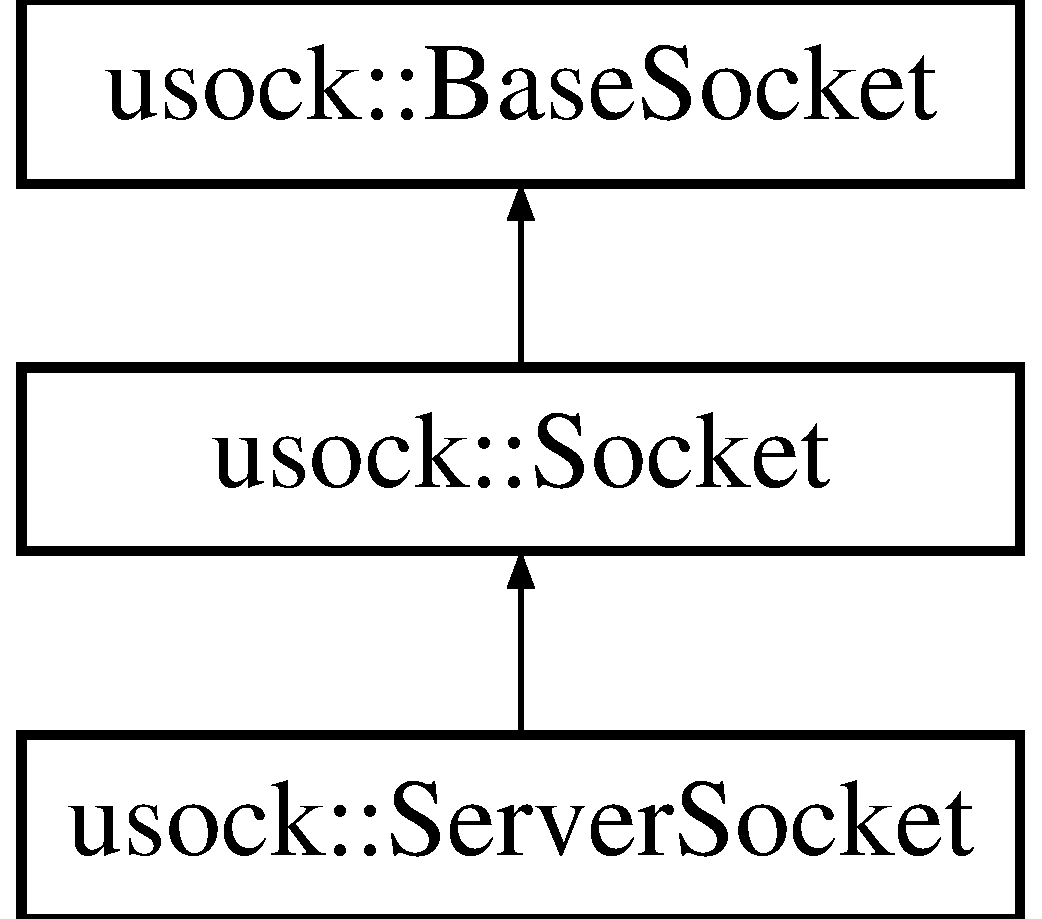
\includegraphics[height=3cm]{classusock_1_1ServerSocket}
\end{center}
\end{figure}
\subsection*{Public Member Functions}
\begin{CompactItemize}
\item 
\hyperlink{classusock_1_1ServerSocket_0ac1908d4a4afb675715ae0ad994e870}{ServerSocket} (u\_\-int16\_\-t port, u\_\-int32\_\-t m=DEFAULT\_\-MAXCON, const std::string \&addr=\char`\"{}\char`\"{})  throw ()
\begin{CompactList}\small\item\em \hyperlink{classusock_1_1ServerSocket}{ServerSocket} high-level constructor. \item\end{CompactList}\item 
\hyperlink{classusock_1_1Socket}{Socket} \hyperlink{classusock_1_1ServerSocket_bf0477af52a725ced6afad86d7b3e794}{accept} ()  throw ()
\begin{CompactList}\small\item\em Wrap around \hyperlink{classusock_1_1ServerSocket_bf0477af52a725ced6afad86d7b3e794}{accept()} function. \item\end{CompactList}\item 
void \hyperlink{classusock_1_1ServerSocket_9ecf37cae8379df6eaf366ab88df244a}{bind} (u\_\-int16\_\-t port)  throw ()
\begin{CompactList}\small\item\em Bind \hyperlink{classusock_1_1ServerSocket}{ServerSocket} onto a port. \item\end{CompactList}\item 
void \hyperlink{classusock_1_1ServerSocket_c6cd2070380b84275c5f69265c57713b}{listen} ()  throw ()
\begin{CompactList}\small\item\em Wrap around \hyperlink{classusock_1_1ServerSocket_c6cd2070380b84275c5f69265c57713b}{listen()} function. \item\end{CompactList}\end{CompactItemize}


\subsection{Detailed Description}
Class for managing TCP server sockets. 

\begin{Desc}
\item[Author:]BlackLight \end{Desc}


\subsection{Constructor \& Destructor Documentation}
\hypertarget{classusock_1_1ServerSocket_0ac1908d4a4afb675715ae0ad994e870}{
\index{usock::ServerSocket@{usock::ServerSocket}!ServerSocket@{ServerSocket}}
\index{ServerSocket@{ServerSocket}!usock::ServerSocket@{usock::ServerSocket}}
\subsubsection[{ServerSocket}]{\setlength{\rightskip}{0pt plus 5cm}usock::ServerSocket::ServerSocket (u\_\-int16\_\-t {\em port}, \/  u\_\-int32\_\-t {\em m} = {\tt DEFAULT\_\-MAXCON}, \/  const std::string \& {\em addr} = {\tt \char`\"{}\char`\"{}})  throw ()}}
\label{classusock_1_1ServerSocket_0ac1908d4a4afb675715ae0ad994e870}


\hyperlink{classusock_1_1ServerSocket}{ServerSocket} high-level constructor. 

\begin{Desc}
\item[Parameters:]
\begin{description}
\item[{\em port}]Port the server will listen onto \item[{\em m}]Maximum number of allowed connections (default = DEFAULT\_\-MAXCON) \item[{\em addr}]Address the socket will listen from, as string (default = INADDR\_\-ANY) \end{description}
\end{Desc}


\subsection{Member Function Documentation}
\hypertarget{classusock_1_1ServerSocket_bf0477af52a725ced6afad86d7b3e794}{
\index{usock::ServerSocket@{usock::ServerSocket}!accept@{accept}}
\index{accept@{accept}!usock::ServerSocket@{usock::ServerSocket}}
\subsubsection[{accept}]{\setlength{\rightskip}{0pt plus 5cm}{\bf Socket} usock::ServerSocket::accept ()  throw ()}}
\label{classusock_1_1ServerSocket_bf0477af52a725ced6afad86d7b3e794}


Wrap around \hyperlink{classusock_1_1ServerSocket_bf0477af52a725ced6afad86d7b3e794}{accept()} function. 

\begin{Desc}
\item[Returns:]A \hyperlink{classusock_1_1Socket}{Socket} object identifying the client connection, if successfully built \end{Desc}
\hypertarget{classusock_1_1ServerSocket_9ecf37cae8379df6eaf366ab88df244a}{
\index{usock::ServerSocket@{usock::ServerSocket}!bind@{bind}}
\index{bind@{bind}!usock::ServerSocket@{usock::ServerSocket}}
\subsubsection[{bind}]{\setlength{\rightskip}{0pt plus 5cm}void usock::ServerSocket::bind (u\_\-int16\_\-t {\em port})  throw ()}}
\label{classusock_1_1ServerSocket_9ecf37cae8379df6eaf366ab88df244a}


Bind \hyperlink{classusock_1_1ServerSocket}{ServerSocket} onto a port. 

\begin{Desc}
\item[Parameters:]
\begin{description}
\item[{\em port}]Port \end{description}
\end{Desc}
\hypertarget{classusock_1_1ServerSocket_c6cd2070380b84275c5f69265c57713b}{
\index{usock::ServerSocket@{usock::ServerSocket}!listen@{listen}}
\index{listen@{listen}!usock::ServerSocket@{usock::ServerSocket}}
\subsubsection[{listen}]{\setlength{\rightskip}{0pt plus 5cm}void usock::ServerSocket::listen ()  throw ()}}
\label{classusock_1_1ServerSocket_c6cd2070380b84275c5f69265c57713b}


Wrap around \hyperlink{classusock_1_1ServerSocket_c6cd2070380b84275c5f69265c57713b}{listen()} function. 



The documentation for this class was generated from the following file:\begin{CompactItemize}
\item 
\hyperlink{usock_8h}{usock.h}\end{CompactItemize}

\hypertarget{classusock_1_1Socket}{
\section{usock::Socket Class Reference}
\label{classusock_1_1Socket}\index{usock::Socket@{usock::Socket}}
}
Class for building TCP sockets.  


{\tt \#include $<$usock.h$>$}

Inheritance diagram for usock::Socket::\begin{figure}[H]
\begin{center}
\leavevmode
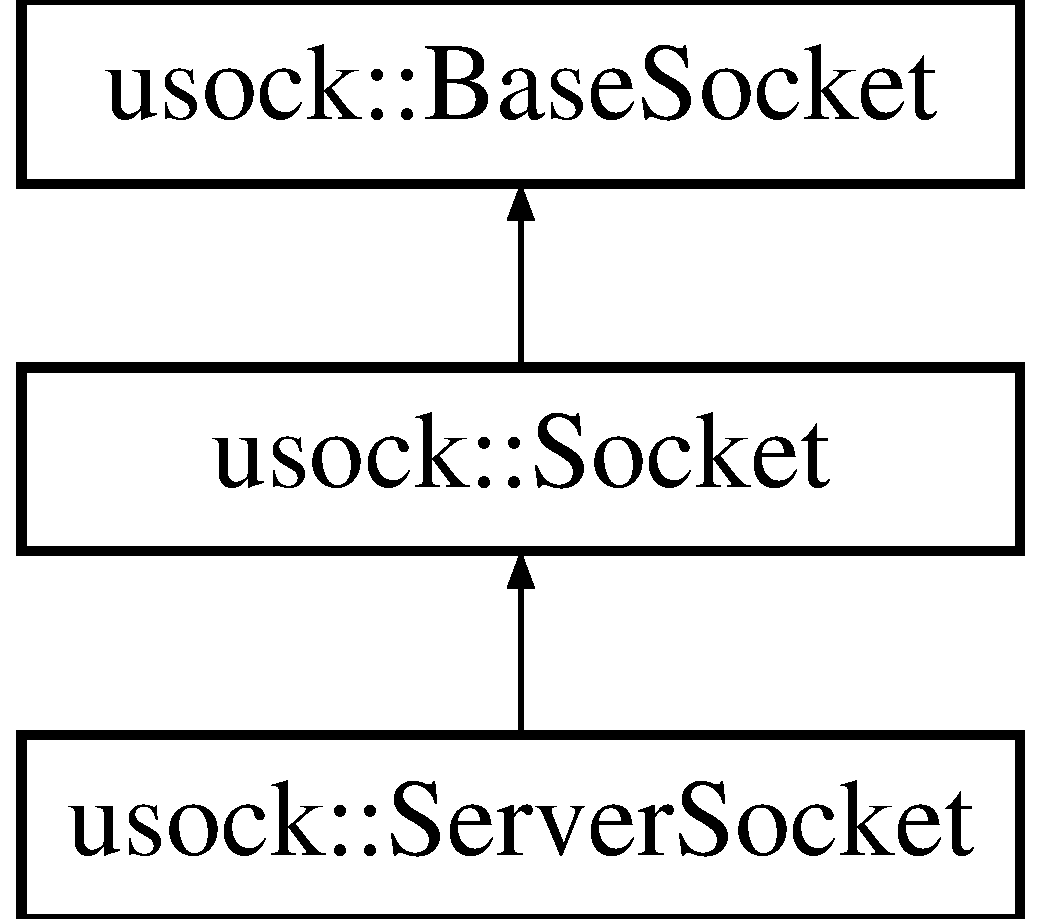
\includegraphics[height=3cm]{classusock_1_1Socket}
\end{center}
\end{figure}
\subsection*{Public Member Functions}
\begin{CompactItemize}
\item 
\hyperlink{classusock_1_1Socket_41721da25729d31889ad3b3312da8532}{Socket} ()  throw ()
\begin{CompactList}\small\item\em Constructor for the \hyperlink{classusock_1_1Socket}{Socket} class. \item\end{CompactList}\item 
\hyperlink{classusock_1_1Socket_157cd31365e1b52709a4abc2c9d7eb05}{Socket} (int \hyperlink{classusock_1_1BaseSocket_63b6c07fb14f937056148cbf8b3531c5}{sd}, double \hyperlink{classusock_1_1BaseSocket_b419e8fd0b849c74b73a02d6bd9081e3}{timeout}=0.0)  throw ()
\begin{CompactList}\small\item\em Constructor for the \hyperlink{classusock_1_1Socket}{Socket} class using an already existent socket descriptor. \item\end{CompactList}\item 
\hyperlink{classusock_1_1Socket_12fa74b5a9eebcea247aa00a1236c0ee}{Socket} (const std::string \&host, u\_\-int16\_\-t port, double \hyperlink{classusock_1_1BaseSocket_b419e8fd0b849c74b73a02d6bd9081e3}{timeout}=0.0)  throw ()
\begin{CompactList}\small\item\em Constructor for the \hyperlink{classusock_1_1Socket}{Socket} class, builds a TCP socket and connects onto it. \item\end{CompactList}\item 
void \hyperlink{classusock_1_1Socket_2036f820d8973a3e4a7cd9c60d6a5a24}{connect} (const std::string \&host, u\_\-int16\_\-t port)  throw ()
\begin{CompactList}\small\item\em Create a TCP connection on the socket. \item\end{CompactList}\item 
void \hyperlink{classusock_1_1Socket_6aa18c3c0131c826afe790a4c8c7aa77}{send} (const std::string \&buf)  throw ()
\begin{CompactList}\small\item\em Send a string onto a TCP socket. \item\end{CompactList}\item 
void \hyperlink{classusock_1_1Socket_a42fa11f66d5f75f37c67f3a31d1ea81}{send} (const void $\ast$buf, u\_\-int32\_\-t size)  throw ()
\begin{CompactList}\small\item\em Send a binary buffer onto a TCP socket. \item\end{CompactList}\item 
void \hyperlink{classusock_1_1Socket_07ccbad3e0d485df8111aec584c2f38e}{operator$<$$<$} (const char \&buf)  throw ()
\begin{CompactList}\small\item\em Overloaded operator to send a buffer onto a TCP socket. \item\end{CompactList}\item 
void \hyperlink{classusock_1_1Socket_41c1bddf8c1cc6bf2b7c06d9da38ebad}{operator$<$$<$} (const int \&buf)  throw ()
\item 
void \hyperlink{classusock_1_1Socket_da103da3dcc47ab072efd471deb4aa17}{operator$<$$<$} (const float \&buf)  throw ()
\item 
void \hyperlink{classusock_1_1Socket_b1da84bc5e90631c85b85e12852b5399}{operator$<$$<$} (const double \&buf)  throw ()
\item 
void \hyperlink{classusock_1_1Socket_1887be63ebc540949cfadf18fa5d9532}{operator$<$$<$} (const std::string \&buf)  throw ()
\item 
void \hyperlink{classusock_1_1Socket_9796319ece2e7d7f7463608f00413457}{operator$>$$>$} (std::string \&buf)  throw ()
\begin{CompactList}\small\item\em Overloaded operator to receive a buffer from a socket (default size: BUFRECV\_\-SIZE). \item\end{CompactList}\item 
std::string \hyperlink{classusock_1_1Socket_be79db8987d9d0dd3a534fca7a84f0f9}{recv} (u\_\-int32\_\-t nbytes=BUFRECV\_\-SIZE)  throw ()
\begin{CompactList}\small\item\em Receive a buffer from a TCP socket. \item\end{CompactList}\item 
void \hyperlink{classusock_1_1Socket_852c343031c5516f747577ee6f3fc96e}{recv} (void $\ast$buf, u\_\-int32\_\-t size)  throw ()
\begin{CompactList}\small\item\em Receive a binary buffer from a TCP socket. \item\end{CompactList}\item 
std::string \hyperlink{classusock_1_1Socket_179bbc1c0b837c0e73c22c1b9bc149eb}{readline} ()  throw ()
\begin{CompactList}\small\item\em Read an ASCII line from the socket. \item\end{CompactList}\end{CompactItemize}


\subsection{Detailed Description}
Class for building TCP sockets. 

\begin{Desc}
\item[Author:]BlackLight \end{Desc}


\subsection{Constructor \& Destructor Documentation}
\hypertarget{classusock_1_1Socket_41721da25729d31889ad3b3312da8532}{
\index{usock::Socket@{usock::Socket}!Socket@{Socket}}
\index{Socket@{Socket}!usock::Socket@{usock::Socket}}
\subsubsection[{Socket}]{\setlength{\rightskip}{0pt plus 5cm}usock::Socket::Socket ()  throw ()}}
\label{classusock_1_1Socket_41721da25729d31889ad3b3312da8532}


Constructor for the \hyperlink{classusock_1_1Socket}{Socket} class. 

\hypertarget{classusock_1_1Socket_157cd31365e1b52709a4abc2c9d7eb05}{
\index{usock::Socket@{usock::Socket}!Socket@{Socket}}
\index{Socket@{Socket}!usock::Socket@{usock::Socket}}
\subsubsection[{Socket}]{\setlength{\rightskip}{0pt plus 5cm}usock::Socket::Socket (int {\em sd}, \/  double {\em timeout} = {\tt 0.0})  throw ()}}
\label{classusock_1_1Socket_157cd31365e1b52709a4abc2c9d7eb05}


Constructor for the \hyperlink{classusock_1_1Socket}{Socket} class using an already existent socket descriptor. 

\begin{Desc}
\item[Parameters:]
\begin{description}
\item[{\em sd}]\hyperlink{classusock_1_1Socket}{Socket} descriptor \item[{\em timeout}]Timeout to be set on the socket \end{description}
\end{Desc}
\hypertarget{classusock_1_1Socket_12fa74b5a9eebcea247aa00a1236c0ee}{
\index{usock::Socket@{usock::Socket}!Socket@{Socket}}
\index{Socket@{Socket}!usock::Socket@{usock::Socket}}
\subsubsection[{Socket}]{\setlength{\rightskip}{0pt plus 5cm}usock::Socket::Socket (const std::string \& {\em host}, \/  u\_\-int16\_\-t {\em port}, \/  double {\em timeout} = {\tt 0.0})  throw ()}}
\label{classusock_1_1Socket_12fa74b5a9eebcea247aa00a1236c0ee}


Constructor for the \hyperlink{classusock_1_1Socket}{Socket} class, builds a TCP socket and connects onto it. 

\begin{Desc}
\item[Parameters:]
\begin{description}
\item[{\em host}]Host name/address \item[{\em port}]Remote port \item[{\em timeout}]Timeout to be set on the socket \end{description}
\end{Desc}


\subsection{Member Function Documentation}
\hypertarget{classusock_1_1Socket_2036f820d8973a3e4a7cd9c60d6a5a24}{
\index{usock::Socket@{usock::Socket}!connect@{connect}}
\index{connect@{connect}!usock::Socket@{usock::Socket}}
\subsubsection[{connect}]{\setlength{\rightskip}{0pt plus 5cm}void usock::Socket::connect (const std::string \& {\em host}, \/  u\_\-int16\_\-t {\em port})  throw ()}}
\label{classusock_1_1Socket_2036f820d8973a3e4a7cd9c60d6a5a24}


Create a TCP connection on the socket. 

\begin{Desc}
\item[Parameters:]
\begin{description}
\item[{\em host}]Host name/address \item[{\em port}]Remote port \end{description}
\end{Desc}
\hypertarget{classusock_1_1Socket_1887be63ebc540949cfadf18fa5d9532}{
\index{usock::Socket@{usock::Socket}!operator$<$$<$@{operator$<$$<$}}
\index{operator$<$$<$@{operator$<$$<$}!usock::Socket@{usock::Socket}}
\subsubsection[{operator$<$$<$}]{\setlength{\rightskip}{0pt plus 5cm}void usock::Socket::operator$<$$<$ (const std::string \& {\em buf})  throw ()}}
\label{classusock_1_1Socket_1887be63ebc540949cfadf18fa5d9532}


\hypertarget{classusock_1_1Socket_b1da84bc5e90631c85b85e12852b5399}{
\index{usock::Socket@{usock::Socket}!operator$<$$<$@{operator$<$$<$}}
\index{operator$<$$<$@{operator$<$$<$}!usock::Socket@{usock::Socket}}
\subsubsection[{operator$<$$<$}]{\setlength{\rightskip}{0pt plus 5cm}void usock::Socket::operator$<$$<$ (const double \& {\em buf})  throw ()}}
\label{classusock_1_1Socket_b1da84bc5e90631c85b85e12852b5399}


\hypertarget{classusock_1_1Socket_da103da3dcc47ab072efd471deb4aa17}{
\index{usock::Socket@{usock::Socket}!operator$<$$<$@{operator$<$$<$}}
\index{operator$<$$<$@{operator$<$$<$}!usock::Socket@{usock::Socket}}
\subsubsection[{operator$<$$<$}]{\setlength{\rightskip}{0pt plus 5cm}void usock::Socket::operator$<$$<$ (const float \& {\em buf})  throw ()}}
\label{classusock_1_1Socket_da103da3dcc47ab072efd471deb4aa17}


\hypertarget{classusock_1_1Socket_41c1bddf8c1cc6bf2b7c06d9da38ebad}{
\index{usock::Socket@{usock::Socket}!operator$<$$<$@{operator$<$$<$}}
\index{operator$<$$<$@{operator$<$$<$}!usock::Socket@{usock::Socket}}
\subsubsection[{operator$<$$<$}]{\setlength{\rightskip}{0pt plus 5cm}void usock::Socket::operator$<$$<$ (const int \& {\em buf})  throw ()}}
\label{classusock_1_1Socket_41c1bddf8c1cc6bf2b7c06d9da38ebad}


\hypertarget{classusock_1_1Socket_07ccbad3e0d485df8111aec584c2f38e}{
\index{usock::Socket@{usock::Socket}!operator$<$$<$@{operator$<$$<$}}
\index{operator$<$$<$@{operator$<$$<$}!usock::Socket@{usock::Socket}}
\subsubsection[{operator$<$$<$}]{\setlength{\rightskip}{0pt plus 5cm}void usock::Socket::operator$<$$<$ (const char \& {\em buf})  throw ()}}
\label{classusock_1_1Socket_07ccbad3e0d485df8111aec584c2f38e}


Overloaded operator to send a buffer onto a TCP socket. 

\begin{Desc}
\item[Parameters:]
\begin{description}
\item[{\em buf}]Stuff to be sent \end{description}
\end{Desc}
\hypertarget{classusock_1_1Socket_9796319ece2e7d7f7463608f00413457}{
\index{usock::Socket@{usock::Socket}!operator$>$$>$@{operator$>$$>$}}
\index{operator$>$$>$@{operator$>$$>$}!usock::Socket@{usock::Socket}}
\subsubsection[{operator$>$$>$}]{\setlength{\rightskip}{0pt plus 5cm}void usock::Socket::operator$>$$>$ (std::string \& {\em buf})  throw ()}}
\label{classusock_1_1Socket_9796319ece2e7d7f7463608f00413457}


Overloaded operator to receive a buffer from a socket (default size: BUFRECV\_\-SIZE). 

\begin{Desc}
\item[Parameters:]
\begin{description}
\item[{\em buf}]String object where we're going to put our received stuff \end{description}
\end{Desc}
\hypertarget{classusock_1_1Socket_179bbc1c0b837c0e73c22c1b9bc149eb}{
\index{usock::Socket@{usock::Socket}!readline@{readline}}
\index{readline@{readline}!usock::Socket@{usock::Socket}}
\subsubsection[{readline}]{\setlength{\rightskip}{0pt plus 5cm}std::string usock::Socket::readline ()  throw ()}}
\label{classusock_1_1Socket_179bbc1c0b837c0e73c22c1b9bc149eb}


Read an ASCII line from the socket. 

\begin{Desc}
\item[Returns:]String containing the read line \end{Desc}
\hypertarget{classusock_1_1Socket_852c343031c5516f747577ee6f3fc96e}{
\index{usock::Socket@{usock::Socket}!recv@{recv}}
\index{recv@{recv}!usock::Socket@{usock::Socket}}
\subsubsection[{recv}]{\setlength{\rightskip}{0pt plus 5cm}void usock::Socket::recv (void $\ast$ {\em buf}, \/  u\_\-int32\_\-t {\em size})  throw ()}}
\label{classusock_1_1Socket_852c343031c5516f747577ee6f3fc96e}


Receive a binary buffer from a TCP socket. 

\begin{Desc}
\item[Parameters:]
\begin{description}
\item[{\em buf}]Buffer where the read stuff will be placed \item[{\em size}]Number of bytes to be read \end{description}
\end{Desc}
\hypertarget{classusock_1_1Socket_be79db8987d9d0dd3a534fca7a84f0f9}{
\index{usock::Socket@{usock::Socket}!recv@{recv}}
\index{recv@{recv}!usock::Socket@{usock::Socket}}
\subsubsection[{recv}]{\setlength{\rightskip}{0pt plus 5cm}std::string usock::Socket::recv (u\_\-int32\_\-t {\em nbytes} = {\tt BUFRECV\_\-SIZE})  throw ()}}
\label{classusock_1_1Socket_be79db8987d9d0dd3a534fca7a84f0f9}


Receive a buffer from a TCP socket. 

\begin{Desc}
\item[Parameters:]
\begin{description}
\item[{\em nbytes}]Number of bytes to be read \end{description}
\end{Desc}
\begin{Desc}
\item[Returns:]A string containing the bytes read from the socket \end{Desc}
\hypertarget{classusock_1_1Socket_a42fa11f66d5f75f37c67f3a31d1ea81}{
\index{usock::Socket@{usock::Socket}!send@{send}}
\index{send@{send}!usock::Socket@{usock::Socket}}
\subsubsection[{send}]{\setlength{\rightskip}{0pt plus 5cm}void usock::Socket::send (const void $\ast$ {\em buf}, \/  u\_\-int32\_\-t {\em size})  throw ()}}
\label{classusock_1_1Socket_a42fa11f66d5f75f37c67f3a31d1ea81}


Send a binary buffer onto a TCP socket. 

\begin{Desc}
\item[Parameters:]
\begin{description}
\item[{\em buf}]Buffer to be sent \item[{\em size}]buf's size \end{description}
\end{Desc}
\hypertarget{classusock_1_1Socket_6aa18c3c0131c826afe790a4c8c7aa77}{
\index{usock::Socket@{usock::Socket}!send@{send}}
\index{send@{send}!usock::Socket@{usock::Socket}}
\subsubsection[{send}]{\setlength{\rightskip}{0pt plus 5cm}void usock::Socket::send (const std::string \& {\em buf})  throw ()}}
\label{classusock_1_1Socket_6aa18c3c0131c826afe790a4c8c7aa77}


Send a string onto a TCP socket. 

\begin{Desc}
\item[Parameters:]
\begin{description}
\item[{\em buf}]String to send \end{description}
\end{Desc}


The documentation for this class was generated from the following file:\begin{CompactItemize}
\item 
\hyperlink{usock_8h}{usock.h}\end{CompactItemize}

\hypertarget{classusock_1_1SocketException}{
\section{usock::SocketException Class Reference}
\label{classusock_1_1SocketException}\index{usock::SocketException@{usock::SocketException}}
}
Class for managing exceptions in \hyperlink{namespaceusock}{usock} class.  


{\tt \#include $<$usock\_\-exception.h$>$}

Inherits std::exception.

\subsection*{Public Member Functions}
\begin{CompactItemize}
\item 
\hyperlink{classusock_1_1SocketException_070830054f67291432f897e77bd9be48}{SocketException} (const char $\ast$str)
\item 
const char $\ast$ \hyperlink{classusock_1_1SocketException_8ad4730be89374b7ee56d56b2617f7a1}{what} () const   throw ()
\end{CompactItemize}


\subsection{Detailed Description}
Class for managing exceptions in \hyperlink{namespaceusock}{usock} class. 

\begin{Desc}
\item[Author:]BlackLight \end{Desc}


\subsection{Constructor \& Destructor Documentation}
\hypertarget{classusock_1_1SocketException_070830054f67291432f897e77bd9be48}{
\index{usock::SocketException@{usock::SocketException}!SocketException@{SocketException}}
\index{SocketException@{SocketException}!usock::SocketException@{usock::SocketException}}
\subsubsection[{SocketException}]{\setlength{\rightskip}{0pt plus 5cm}usock::SocketException::SocketException (const char $\ast$ {\em str})\hspace{0.3cm}{\tt  \mbox{[}inline\mbox{]}}}}
\label{classusock_1_1SocketException_070830054f67291432f897e77bd9be48}




\subsection{Member Function Documentation}
\hypertarget{classusock_1_1SocketException_8ad4730be89374b7ee56d56b2617f7a1}{
\index{usock::SocketException@{usock::SocketException}!what@{what}}
\index{what@{what}!usock::SocketException@{usock::SocketException}}
\subsubsection[{what}]{\setlength{\rightskip}{0pt plus 5cm}const char$\ast$ usock::SocketException::what () const  throw ()\hspace{0.3cm}{\tt  \mbox{[}inline\mbox{]}}}}
\label{classusock_1_1SocketException_8ad4730be89374b7ee56d56b2617f7a1}




The documentation for this class was generated from the following file:\begin{CompactItemize}
\item 
\hyperlink{usock__exception_8h}{usock\_\-exception.h}\end{CompactItemize}

\hypertarget{classusock_1_1UDPSocket}{
\section{usock::UDPSocket Class Reference}
\label{classusock_1_1UDPSocket}\index{usock::UDPSocket@{usock::UDPSocket}}
}
Class for managing UDP sockets.  


{\tt \#include $<$usock.h$>$}

Inheritance diagram for usock::UDPSocket::\begin{figure}[H]
\begin{center}
\leavevmode
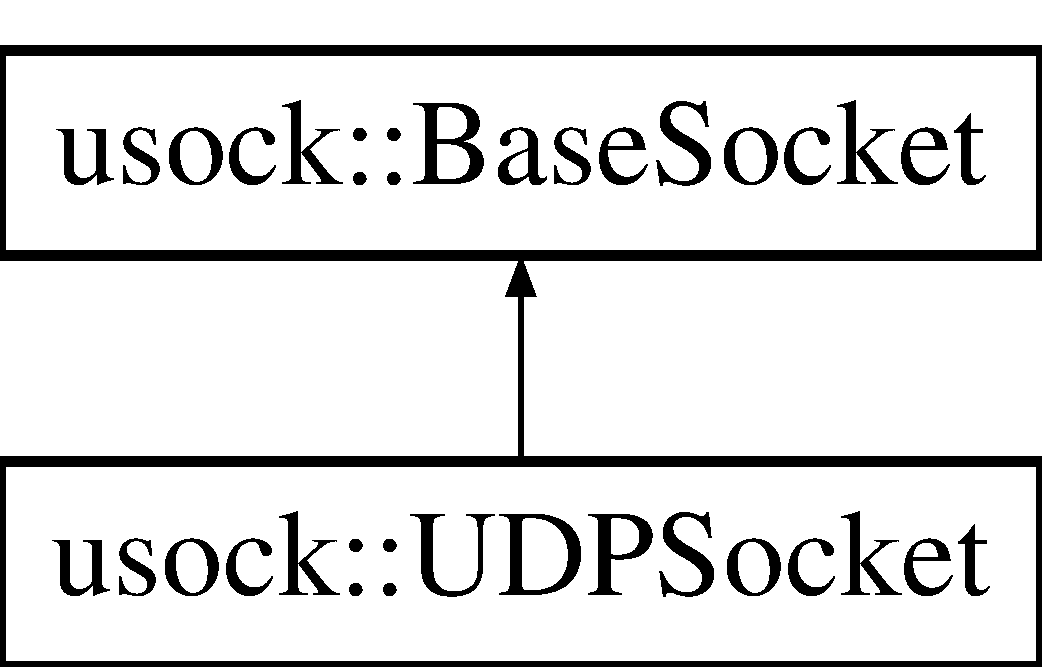
\includegraphics[height=2cm]{classusock_1_1UDPSocket}
\end{center}
\end{figure}
\subsection*{Public Member Functions}
\begin{CompactItemize}
\item 
\hyperlink{classusock_1_1UDPSocket_f1db79ca3083ee144302c2ad9fc1b017}{UDPSocket} (int \hyperlink{classusock_1_1BaseSocket_8117d25c7b482eb594d68137868ce5f9}{type}=AF\_\-INET)  throw ()
\begin{CompactList}\small\item\em \hyperlink{classusock_1_1UDPSocket}{UDPSocket} constructor. \item\end{CompactList}\item 
void \hyperlink{classusock_1_1UDPSocket_5669548bd12ad139cc7b901cb4701e5c}{send} (const std::string \&buf, const std::string \&host, u\_\-int16\_\-t port)  throw ()
\begin{CompactList}\small\item\em Send a string onto an UDP socket. \item\end{CompactList}\item 
void \hyperlink{classusock_1_1UDPSocket_49d2828223835e216fdee794519b00e7}{send} (const void $\ast$buf, u\_\-int32\_\-t size, const std::string \&host, u\_\-int16\_\-t port)  throw ()
\begin{CompactList}\small\item\em Send a binary buffer onto an UDP socket. \item\end{CompactList}\item 
void \hyperlink{classusock_1_1UDPSocket_daab178fe0b22f862e8d25d268080f05}{bind} (u\_\-int16\_\-t port)  throw ()
\begin{CompactList}\small\item\em Bind an UDP socket onto a port. \item\end{CompactList}\item 
void \hyperlink{classusock_1_1UDPSocket_a3ffe1666074dc785e0c70e0d36c9bf4}{recv} (void $\ast$buf, u\_\-int32\_\-t size, const std::string \&host=\char`\"{}\char`\"{}, u\_\-int16\_\-t port=0)  throw ()
\begin{CompactList}\small\item\em Receive a binary buffer from an UDP socket. \item\end{CompactList}\item 
std::string \hyperlink{classusock_1_1UDPSocket_d6dec5293e2768a42b833fb42a720d22}{recv} (const std::string \&host=\char`\"{}\char`\"{}, u\_\-int16\_\-t port=0)  throw ()
\begin{CompactList}\small\item\em Receive an ASCII string from an UDP socket. \item\end{CompactList}\item 
std::string \hyperlink{classusock_1_1UDPSocket_aead0f8a12cc8e98a98473bea4d15a0e}{readline} (const std::string \&host=\char`\"{}\char`\"{}, u\_\-int16\_\-t port=0)  throw ()
\begin{CompactList}\small\item\em Read an ASCII line from an UDP socket. \item\end{CompactList}\end{CompactItemize}


\subsection{Detailed Description}
Class for managing UDP sockets. 

\begin{Desc}
\item[Author:]BlackLight \end{Desc}


\subsection{Constructor \& Destructor Documentation}
\hypertarget{classusock_1_1UDPSocket_f1db79ca3083ee144302c2ad9fc1b017}{
\index{usock::UDPSocket@{usock::UDPSocket}!UDPSocket@{UDPSocket}}
\index{UDPSocket@{UDPSocket}!usock::UDPSocket@{usock::UDPSocket}}
\subsubsection[{UDPSocket}]{\setlength{\rightskip}{0pt plus 5cm}usock::UDPSocket::UDPSocket (int {\em type} = {\tt AF\_\-INET})  throw ()}}
\label{classusock_1_1UDPSocket_f1db79ca3083ee144302c2ad9fc1b017}


\hyperlink{classusock_1_1UDPSocket}{UDPSocket} constructor. 

\begin{Desc}
\item[Parameters:]
\begin{description}
\item[{\em type}]\hyperlink{classusock_1_1Socket}{Socket} type (default = AF\_\-INET) \end{description}
\end{Desc}


\subsection{Member Function Documentation}
\hypertarget{classusock_1_1UDPSocket_daab178fe0b22f862e8d25d268080f05}{
\index{usock::UDPSocket@{usock::UDPSocket}!bind@{bind}}
\index{bind@{bind}!usock::UDPSocket@{usock::UDPSocket}}
\subsubsection[{bind}]{\setlength{\rightskip}{0pt plus 5cm}void usock::UDPSocket::bind (u\_\-int16\_\-t {\em port})  throw ()}}
\label{classusock_1_1UDPSocket_daab178fe0b22f862e8d25d268080f05}


Bind an UDP socket onto a port. 

\begin{Desc}
\item[Parameters:]
\begin{description}
\item[{\em Port}]\end{description}
\end{Desc}
\hypertarget{classusock_1_1UDPSocket_aead0f8a12cc8e98a98473bea4d15a0e}{
\index{usock::UDPSocket@{usock::UDPSocket}!readline@{readline}}
\index{readline@{readline}!usock::UDPSocket@{usock::UDPSocket}}
\subsubsection[{readline}]{\setlength{\rightskip}{0pt plus 5cm}std::string usock::UDPSocket::readline (const std::string \& {\em host} = {\tt \char`\"{}\char`\"{}}, \/  u\_\-int16\_\-t {\em port} = {\tt 0})  throw ()}}
\label{classusock_1_1UDPSocket_aead0f8a12cc8e98a98473bea4d15a0e}


Read an ASCII line from an UDP socket. 

\begin{Desc}
\item[Parameters:]
\begin{description}
\item[{\em host}]Remote host name/address \item[{\em port}]Remote port \end{description}
\end{Desc}
\begin{Desc}
\item[Returns:]String received \end{Desc}
\hypertarget{classusock_1_1UDPSocket_d6dec5293e2768a42b833fb42a720d22}{
\index{usock::UDPSocket@{usock::UDPSocket}!recv@{recv}}
\index{recv@{recv}!usock::UDPSocket@{usock::UDPSocket}}
\subsubsection[{recv}]{\setlength{\rightskip}{0pt plus 5cm}std::string usock::UDPSocket::recv (const std::string \& {\em host} = {\tt \char`\"{}\char`\"{}}, \/  u\_\-int16\_\-t {\em port} = {\tt 0})  throw ()}}
\label{classusock_1_1UDPSocket_d6dec5293e2768a42b833fb42a720d22}


Receive an ASCII string from an UDP socket. 

\begin{Desc}
\item[Parameters:]
\begin{description}
\item[{\em host}]Remote host name/address \item[{\em port}]Remote port \end{description}
\end{Desc}
\begin{Desc}
\item[Returns:]String received \end{Desc}
\hypertarget{classusock_1_1UDPSocket_a3ffe1666074dc785e0c70e0d36c9bf4}{
\index{usock::UDPSocket@{usock::UDPSocket}!recv@{recv}}
\index{recv@{recv}!usock::UDPSocket@{usock::UDPSocket}}
\subsubsection[{recv}]{\setlength{\rightskip}{0pt plus 5cm}void usock::UDPSocket::recv (void $\ast$ {\em buf}, \/  u\_\-int32\_\-t {\em size}, \/  const std::string \& {\em host} = {\tt \char`\"{}\char`\"{}}, \/  u\_\-int16\_\-t {\em port} = {\tt 0})  throw ()}}
\label{classusock_1_1UDPSocket_a3ffe1666074dc785e0c70e0d36c9bf4}


Receive a binary buffer from an UDP socket. 

\begin{Desc}
\item[Parameters:]
\begin{description}
\item[{\em buf}]Buffer where we're going to place our data \item[{\em size}]Number of bytes to be read \item[{\em host}]Remote host name/address \item[{\em port}]Remote port \end{description}
\end{Desc}
\hypertarget{classusock_1_1UDPSocket_49d2828223835e216fdee794519b00e7}{
\index{usock::UDPSocket@{usock::UDPSocket}!send@{send}}
\index{send@{send}!usock::UDPSocket@{usock::UDPSocket}}
\subsubsection[{send}]{\setlength{\rightskip}{0pt plus 5cm}void usock::UDPSocket::send (const void $\ast$ {\em buf}, \/  u\_\-int32\_\-t {\em size}, \/  const std::string \& {\em host}, \/  u\_\-int16\_\-t {\em port})  throw ()}}
\label{classusock_1_1UDPSocket_49d2828223835e216fdee794519b00e7}


Send a binary buffer onto an UDP socket. 

\begin{Desc}
\item[Parameters:]
\begin{description}
\item[{\em buf}]Binary buffer to be sent \item[{\em size}]buf's size \item[{\em host}]Remote host name/address \item[{\em port}]Remote port \end{description}
\end{Desc}
\hypertarget{classusock_1_1UDPSocket_5669548bd12ad139cc7b901cb4701e5c}{
\index{usock::UDPSocket@{usock::UDPSocket}!send@{send}}
\index{send@{send}!usock::UDPSocket@{usock::UDPSocket}}
\subsubsection[{send}]{\setlength{\rightskip}{0pt plus 5cm}void usock::UDPSocket::send (const std::string \& {\em buf}, \/  const std::string \& {\em host}, \/  u\_\-int16\_\-t {\em port})  throw ()}}
\label{classusock_1_1UDPSocket_5669548bd12ad139cc7b901cb4701e5c}


Send a string onto an UDP socket. 

\begin{Desc}
\item[Parameters:]
\begin{description}
\item[{\em buf}]String to be sent \item[{\em host}]Remote host name/address \item[{\em port}]Remote port \end{description}
\end{Desc}


The documentation for this class was generated from the following file:\begin{CompactItemize}
\item 
\hyperlink{usock_8h}{usock.h}\end{CompactItemize}

\chapter{File Documentation}
\hypertarget{usock_8h}{
\section{usock.h File Reference}
\label{usock_8h}\index{usock.h@{usock.h}}
}
{\tt \#include $<$iostream$>$}\par
{\tt \#include $<$sstream$>$}\par
{\tt \#include $<$string$>$}\par
{\tt \#include $<$cstdio$>$}\par
{\tt \#include $<$cstdlib$>$}\par
{\tt \#include $<$ctime$>$}\par
{\tt \#include $<$netinet/in.h$>$}\par
{\tt \#include $<$sys/socket.h$>$}\par
{\tt \#include $<$sys/ioctl.h$>$}\par
{\tt \#include $<$sys/types.h$>$}\par
{\tt \#include $<$arpa/inet.h$>$}\par
{\tt \#include $<$fcntl.h$>$}\par
{\tt \#include $<$netdb.h$>$}\par
{\tt \#include $<$net/if.h$>$}\par
{\tt \#include $<$net/ethernet.h$>$}\par
{\tt \#include $<$netpacket/packet.h$>$}\par
{\tt \#include $<$netinet/ip.h$>$}\par
{\tt \#include $<$netinet/ip6.h$>$}\par
{\tt \#include $<$netinet/ip\_\-icmp.h$>$}\par
{\tt \#include $<$netinet/tcp.h$>$}\par
{\tt \#include $<$netinet/udp.h$>$}\par
\subsection*{Classes}
\begin{CompactItemize}
\item 
struct \hyperlink{structicmp__hdr}{icmp\_\-hdr}
\item 
struct \hyperlink{structpseudohdr}{pseudohdr}
\item 
class \hyperlink{classSocket}{Socket}
\begin{CompactList}\small\item\em Base socket class for building, by default, TCP sockets. \item\end{CompactList}\item 
class \hyperlink{classServerSocket}{ServerSocket}
\begin{CompactList}\small\item\em Class for managing server sockets. \item\end{CompactList}\item 
class \hyperlink{classUDPSocket}{UDPSocket}
\begin{CompactList}\small\item\em Class for managing UDP sockets. \item\end{CompactList}\item 
class \hyperlink{classRawSocket}{RawSocket}
\begin{CompactList}\small\item\em Class for managing raw sockets. \item\end{CompactList}\end{CompactItemize}
\subsection*{Defines}
\begin{CompactItemize}
\item 
\#define \hyperlink{usock_8h_29d0df17f4d361506734c2083f200ea3}{BUFRECV\_\-SIZE}~1024
\item 
\#define \hyperlink{usock_8h_fb2b62b61a722c73b8b798f010063863}{DEFAULT\_\-MAXCON}~10
\item 
\#define \hyperlink{usock_8h_1cec9b372679734fcd8394d779442ddb}{TH\_\-FIN}~0x01
\item 
\#define \hyperlink{usock_8h_91006117f7ae427b957773ab0e80bfa4}{TH\_\-SYN}~0x02
\item 
\#define \hyperlink{usock_8h_7f2ce15991898c8d3397045087c4381f}{TH\_\-RST}~0x04
\item 
\#define \hyperlink{usock_8h_45b9964096064c9a0c84fbddd2c80d38}{TH\_\-PUSH}~0x08
\item 
\#define \hyperlink{usock_8h_362dae974cf06bab2b79b70f0cde524f}{TH\_\-ACK}~0x10
\item 
\#define \hyperlink{usock_8h_7b18ca973f14696013696a00c5235f32}{TH\_\-URG}~0x20
\end{CompactItemize}


\subsection{Define Documentation}
\hypertarget{usock_8h_29d0df17f4d361506734c2083f200ea3}{
\index{usock.h@{usock.h}!BUFRECV\_\-SIZE@{BUFRECV\_\-SIZE}}
\index{BUFRECV\_\-SIZE@{BUFRECV\_\-SIZE}!usock.h@{usock.h}}
\subsubsection[{BUFRECV\_\-SIZE}]{\setlength{\rightskip}{0pt plus 5cm}\#define BUFRECV\_\-SIZE~1024}}
\label{usock_8h_29d0df17f4d361506734c2083f200ea3}


\hypertarget{usock_8h_fb2b62b61a722c73b8b798f010063863}{
\index{usock.h@{usock.h}!DEFAULT\_\-MAXCON@{DEFAULT\_\-MAXCON}}
\index{DEFAULT\_\-MAXCON@{DEFAULT\_\-MAXCON}!usock.h@{usock.h}}
\subsubsection[{DEFAULT\_\-MAXCON}]{\setlength{\rightskip}{0pt plus 5cm}\#define DEFAULT\_\-MAXCON~10}}
\label{usock_8h_fb2b62b61a722c73b8b798f010063863}


\hypertarget{usock_8h_362dae974cf06bab2b79b70f0cde524f}{
\index{usock.h@{usock.h}!TH\_\-ACK@{TH\_\-ACK}}
\index{TH\_\-ACK@{TH\_\-ACK}!usock.h@{usock.h}}
\subsubsection[{TH\_\-ACK}]{\setlength{\rightskip}{0pt plus 5cm}\#define TH\_\-ACK~0x10}}
\label{usock_8h_362dae974cf06bab2b79b70f0cde524f}


\hypertarget{usock_8h_1cec9b372679734fcd8394d779442ddb}{
\index{usock.h@{usock.h}!TH\_\-FIN@{TH\_\-FIN}}
\index{TH\_\-FIN@{TH\_\-FIN}!usock.h@{usock.h}}
\subsubsection[{TH\_\-FIN}]{\setlength{\rightskip}{0pt plus 5cm}\#define TH\_\-FIN~0x01}}
\label{usock_8h_1cec9b372679734fcd8394d779442ddb}


\hypertarget{usock_8h_45b9964096064c9a0c84fbddd2c80d38}{
\index{usock.h@{usock.h}!TH\_\-PUSH@{TH\_\-PUSH}}
\index{TH\_\-PUSH@{TH\_\-PUSH}!usock.h@{usock.h}}
\subsubsection[{TH\_\-PUSH}]{\setlength{\rightskip}{0pt plus 5cm}\#define TH\_\-PUSH~0x08}}
\label{usock_8h_45b9964096064c9a0c84fbddd2c80d38}


\hypertarget{usock_8h_7f2ce15991898c8d3397045087c4381f}{
\index{usock.h@{usock.h}!TH\_\-RST@{TH\_\-RST}}
\index{TH\_\-RST@{TH\_\-RST}!usock.h@{usock.h}}
\subsubsection[{TH\_\-RST}]{\setlength{\rightskip}{0pt plus 5cm}\#define TH\_\-RST~0x04}}
\label{usock_8h_7f2ce15991898c8d3397045087c4381f}


\hypertarget{usock_8h_91006117f7ae427b957773ab0e80bfa4}{
\index{usock.h@{usock.h}!TH\_\-SYN@{TH\_\-SYN}}
\index{TH\_\-SYN@{TH\_\-SYN}!usock.h@{usock.h}}
\subsubsection[{TH\_\-SYN}]{\setlength{\rightskip}{0pt plus 5cm}\#define TH\_\-SYN~0x02}}
\label{usock_8h_91006117f7ae427b957773ab0e80bfa4}


\hypertarget{usock_8h_7b18ca973f14696013696a00c5235f32}{
\index{usock.h@{usock.h}!TH\_\-URG@{TH\_\-URG}}
\index{TH\_\-URG@{TH\_\-URG}!usock.h@{usock.h}}
\subsubsection[{TH\_\-URG}]{\setlength{\rightskip}{0pt plus 5cm}\#define TH\_\-URG~0x20}}
\label{usock_8h_7b18ca973f14696013696a00c5235f32}



\hypertarget{usock__exception_8h}{
\section{usock\_\-exception.h File Reference}
\label{usock__exception_8h}\index{usock\_\-exception.h@{usock\_\-exception.h}}
}
{\tt \#include $<$exception$>$}\par
{\tt \#include $<$cerrno$>$}\par
\subsection*{Classes}
\begin{CompactItemize}
\item 
class \hyperlink{classusock_1_1SocketException}{usock::SocketException}
\begin{CompactList}\small\item\em Class for managing exceptions in \hyperlink{namespaceusock}{usock} library. \item\end{CompactList}\end{CompactItemize}
\subsection*{Namespaces}
\begin{CompactItemize}
\item 
namespace \hyperlink{namespaceusock}{usock}
\end{CompactItemize}
\subsection*{Defines}
\begin{CompactItemize}
\item 
\#define \hyperlink{usock__exception_8h_8aa7a302e0160545c42054cfa6e3b743}{ERRBUF\_\-SIZE}~1024
\end{CompactItemize}


\subsection{Define Documentation}
\hypertarget{usock__exception_8h_8aa7a302e0160545c42054cfa6e3b743}{
\index{usock\_\-exception.h@{usock\_\-exception.h}!ERRBUF\_\-SIZE@{ERRBUF\_\-SIZE}}
\index{ERRBUF\_\-SIZE@{ERRBUF\_\-SIZE}!usock_exception.h@{usock\_\-exception.h}}
\subsubsection[{ERRBUF\_\-SIZE}]{\setlength{\rightskip}{0pt plus 5cm}\#define ERRBUF\_\-SIZE~1024}}
\label{usock__exception_8h_8aa7a302e0160545c42054cfa6e3b743}



\printindex
\end{document}
